%!TEX TS-program = xelatex
\documentclass[10pt,oneside]{article}
\usepackage[fontsize=9pt]{scrextend}

\usepackage[english]{babel}

\usepackage{amsmath,amssymb,amsfonts}
\usepackage[utf8]{inputenc}
\usepackage[T1]{fontenc}
\usepackage{stix2}
\usepackage[scaled]{helvet}
\usepackage[scaled]{inconsolata}

\usepackage{lastpage}

\usepackage{setspace}

\usepackage{ccicons}

\usepackage[hang,flushmargin]{footmisc}

\usepackage{geometry}

\setlength{\parindent}{0pt}
\setlength{\parskip}{6pt plus 2pt minus 1pt}

\usepackage{fancyhdr}
\renewcommand{\headrulewidth}{0pt}\providecommand{\tightlist}{%
  \setlength{\itemsep}{0pt}\setlength{\parskip}{0pt}}

\makeatletter
\newcounter{tableno}
\newenvironment{tablenos:no-prefix-table-caption}{
  \caption@ifcompatibility{}{
    \let\oldthetable\thetable
    \let\oldtheHtable\theHtable
    \renewcommand{\thetable}{tableno:\thetableno}
    \renewcommand{\theHtable}{tableno:\thetableno}
    \stepcounter{tableno}
    \captionsetup{labelformat=empty}
  }
}{
  \caption@ifcompatibility{}{
    \captionsetup{labelformat=default}
    \let\thetable\oldthetable
    \let\theHtable\oldtheHtable
    \addtocounter{table}{-1}
  }
}
\makeatother

\usepackage{array}
\newcommand{\PreserveBackslash}[1]{\let\temp=\\#1\let\\=\temp}
\let\PBS=\PreserveBackslash

\usepackage[breaklinks=true]{hyperref}
\hypersetup{colorlinks,%
citecolor=blue,%
filecolor=blue,%
linkcolor=blue,%
urlcolor=blue}
\usepackage{url}

\usepackage{caption}
\setcounter{secnumdepth}{0}
\usepackage{cleveref}

\usepackage{graphicx}
\makeatletter
\def\maxwidth{\ifdim\Gin@nat@width>\linewidth\linewidth
\else\Gin@nat@width\fi}
\makeatother
\let\Oldincludegraphics\includegraphics
\renewcommand{\includegraphics}[1]{\Oldincludegraphics[width=\maxwidth]{#1}}

\usepackage{longtable}
\usepackage{booktabs}

\usepackage{color}
\usepackage{fancyvrb}
\newcommand{\VerbBar}{|}
\newcommand{\VERB}{\Verb[commandchars=\\\{\}]}
\DefineVerbatimEnvironment{Highlighting}{Verbatim}{commandchars=\\\{\}}
% Add ',fontsize=\small' for more characters per line
\usepackage{framed}
\definecolor{shadecolor}{RGB}{248,248,248}
\newenvironment{Shaded}{\begin{snugshade}}{\end{snugshade}}
\newcommand{\KeywordTok}[1]{\textcolor[rgb]{0.13,0.29,0.53}{\textbf{#1}}}
\newcommand{\DataTypeTok}[1]{\textcolor[rgb]{0.13,0.29,0.53}{#1}}
\newcommand{\DecValTok}[1]{\textcolor[rgb]{0.00,0.00,0.81}{#1}}
\newcommand{\BaseNTok}[1]{\textcolor[rgb]{0.00,0.00,0.81}{#1}}
\newcommand{\FloatTok}[1]{\textcolor[rgb]{0.00,0.00,0.81}{#1}}
\newcommand{\ConstantTok}[1]{\textcolor[rgb]{0.00,0.00,0.00}{#1}}
\newcommand{\CharTok}[1]{\textcolor[rgb]{0.31,0.60,0.02}{#1}}
\newcommand{\SpecialCharTok}[1]{\textcolor[rgb]{0.00,0.00,0.00}{#1}}
\newcommand{\StringTok}[1]{\textcolor[rgb]{0.31,0.60,0.02}{#1}}
\newcommand{\VerbatimStringTok}[1]{\textcolor[rgb]{0.31,0.60,0.02}{#1}}
\newcommand{\SpecialStringTok}[1]{\textcolor[rgb]{0.31,0.60,0.02}{#1}}
\newcommand{\ImportTok}[1]{#1}
\newcommand{\CommentTok}[1]{\textcolor[rgb]{0.56,0.35,0.01}{\textit{#1}}}
\newcommand{\DocumentationTok}[1]{\textcolor[rgb]{0.56,0.35,0.01}{\textbf{\textit{#1}}}}
\newcommand{\AnnotationTok}[1]{\textcolor[rgb]{0.56,0.35,0.01}{\textbf{\textit{#1}}}}
\newcommand{\CommentVarTok}[1]{\textcolor[rgb]{0.56,0.35,0.01}{\textbf{\textit{#1}}}}
\newcommand{\OtherTok}[1]{\textcolor[rgb]{0.56,0.35,0.01}{#1}}
\newcommand{\FunctionTok}[1]{\textcolor[rgb]{0.00,0.00,0.00}{#1}}
\newcommand{\VariableTok}[1]{\textcolor[rgb]{0.00,0.00,0.00}{#1}}
\newcommand{\ControlFlowTok}[1]{\textcolor[rgb]{0.13,0.29,0.53}{\textbf{#1}}}
\newcommand{\OperatorTok}[1]{\textcolor[rgb]{0.81,0.36,0.00}{\textbf{#1}}}
\newcommand{\BuiltInTok}[1]{#1}
\newcommand{\ExtensionTok}[1]{#1}
\newcommand{\PreprocessorTok}[1]{\textcolor[rgb]{0.56,0.35,0.01}{\textit{#1}}}
\newcommand{\AttributeTok}[1]{\textcolor[rgb]{0.77,0.63,0.00}{#1}}
\newcommand{\RegionMarkerTok}[1]{#1}
\newcommand{\InformationTok}[1]{\textcolor[rgb]{0.56,0.35,0.01}{\textbf{\textit{#1}}}}
\newcommand{\WarningTok}[1]{\textcolor[rgb]{0.56,0.35,0.01}{\textbf{\textit{#1}}}}
\newcommand{\AlertTok}[1]{\textcolor[rgb]{0.94,0.16,0.16}{#1}}
\newcommand{\ErrorTok}[1]{\textcolor[rgb]{0.64,0.00,0.00}{\textbf{#1}}}
\newcommand{\NormalTok}[1]{#1}

\newlength{\cslhangindent}
\setlength{\cslhangindent}{1.5em}
\newlength{\csllabelwidth}
\setlength{\csllabelwidth}{3em}
\newenvironment{CSLReferences}[3] % #1 hanging-ident, #2 entry spacing
 {% don't indent paragraphs
  \setlength{\parindent}{0pt}
  % turn on hanging indent if param 1 is 1
  \ifodd #1 \everypar{\setlength{\hangindent}{\cslhangindent}}\ignorespaces\fi
  % set entry spacing
  \ifnum #2 > 0
  \setlength{\parskip}{#2\baselineskip}
  \fi
 }%
 {}
\usepackage{calc} % for \widthof, \maxof
\newcommand{\CSLBlock}[1]{#1\hfill\break}
\newcommand{\CSLLeftMargin}[1]{\parbox[t]{\maxof{\widthof{#1}}{\csllabelwidth}}{#1}}
\newcommand{\CSLRightInline}[1]{\parbox[t]{\linewidth}{#1}}
\newcommand{\CSLIndent}[1]{\hspace{\cslhangindent}#1}\usepackage[table,dvipsnames]{xcolor}

\geometry{includemp,
            letterpaper,
            top=2.4cm,
            bottom=2.4cm,
            left=1.0cm,
            right=1.0cm,
            marginparwidth=5cm,
            marginparsep=1.0cm}

\usepackage[singlelinecheck=off]{caption}

\captionsetup{
  font={small},
  labelfont={bf},
  format=plain,
  labelsep=quad
}

\usepackage{floatrow}

\floatsetup[figure]{margins=hangright,
              facing=no,
              capposition=beside,
              capbesideposition={center,outside},
              floatwidth=\textwidth}

% \floatsetup[table]{margins=hangright,
%              facing=no,
%              capposition=beside,
%              capbesideposition={center,outside},
%              floatwidth=\textwidth}

\pagestyle{plain}

\setcounter{secnumdepth}{5}

\usepackage{titlesec}

\titleformat{\section}[block]
{\normalfont\large\sffamily}
{\thesection}{.5em}{\titlerule\\[.8ex]\bfseries}

\titleformat{\subsection}[runin]
{\normalfont\fontseries{b}\selectfont\filright\sffamily}
{\thesubsection.}{.5em}{}

\titleformat{\subsubsection}[runin]
{\normalfont\itshape\rmfamily\bfseries}{\thesubsubsection}{1em}{}

\fancypagestyle{firstpage}
{
   \fancyhf{}
   \renewcommand{\headrulewidth}{0pt}
   \fancyfoot[R]{\footnotesize\ccby}
   \fancyfoot[L]{\footnotesize\sffamily\today}
}

\fancypagestyle{normal}
{
  \fancyhf{}
  \fancyfoot[R]{\footnotesize\sffamily\thepage\ of \pageref*{LastPage}}
}

\usepackage{tikz}
\begin{document}
\tikz [remember picture, overlay] %
\node [shift={(-0.6in,1.1cm)},scale=0.2,opacity=0.4] at (current page.south east)[anchor=south east]{
\includegraphics{logo}};%
\pagestyle{normal}
\thispagestyle{firstpage}

\newcommand{\colorRule}[3][black]{\textcolor[HTML]{#1}{\rule{#2}{#3}}}

\noindent {\LARGE \textbf{\textsf{The coevolutionary mosaic of bat
betacoronavirus emergence risk}}}

\medskip
\begin{flushleft}
{\small
%
Norma R\,Forero-Muñoz%
%
\,\textsuperscript{1,2,‡}, %
Renata L.\,Muylaert%
%
\,\textsuperscript{3}, %
Stephanie N.\,Seifert%
%
\,\textsuperscript{4}, %
Gregory F.\,Albery%
%
\,\textsuperscript{5}, %
Daniel J.\,Becker%
%
\,\textsuperscript{6}, %
Colin J.\,Carlson%
%
\,\textsuperscript{7,8,9,‡}, %
\href{https://orcid.org/0000-0002-0735-5184}{Timothée\,Poisot}%
%
\,\textsuperscript{1,2,‡}
\vskip 1em
\textsuperscript{1}\,Université de Montréal; \textsuperscript{2}\,Québec
Centre for Biodiversity Sciences; \textsuperscript{3}\,Molecular
Epidemiology and Public Health Laboratory, School of Veterinary Science,
Massey University, New Zealand; \textsuperscript{4}\,Paul G. Allen
School for Global Health, Washington State University, Pullman, WA,
United States; \textsuperscript{5}\,Department of Biology, Georgetown
University, Washington, DC, USA; \textsuperscript{6}\,Department of
Biology, University of Oklahoma, Norman, OK,
USA; \textsuperscript{7}\,Department of Biology, Georgetown University,
Washington, DC,; \textsuperscript{8}\,Center for Global Health Science
and Security, Georgetown University Medical Center, Washington, DC,
USA; \textsuperscript{9}\,Department of Microbiology and Immunology,
Georgetown University Medical Center, Washington, DC, USA\\
\textsuperscript{‡}\,These authors contributed equally to the work\\
\vskip 1em
\textbf{Correspondance to:}\\
Timothée Poisot --- \texttt{timothee.poisot@umontreal.ca}\\
}
\end{flushleft}

\vskip 2em
\makebox[0pt][l]{\colorRule[CCCCCC]{2.0\textwidth}{0.5pt}}
\vskip 2em
\noindent

\marginpar{\vskip 1em\flushright
{\small{\bfseries Keywords}:\par
bats\\betacoronavirus\\disease ecology\\geographic mosaic theory of
coevolution\\phylogenetic diversity\\viral sharing\\SARS-CoV-2\\}
}


Pathogen evolution is one of the least predictable components of disease
emergence, particularly in nature. Here, building on principles
established by the geographic mosaic theory of coevolution, we develop a
quantitative, spatially-explicit framework for mapping the evolutionary
risk of viral emergence. Driven by interest in diseases like SARS, MERS,
and COVID-19, we examine the global biogeography of bat-origin
betacoronaviruses, and find that coevolutionary principles suggest
geographies of risk that are distinct from the hotspots and coldspots of
host richness. Further, our framework helps explain patterns like a
unique pool of merbecoviruses in the Neotropics, a recently-discovered
lineage of divergent nobecoviruses in Madagascar, and--most
importantly--hotspots of diversification in southeast Asia, sub-Saharan
Africa, and the Middle East that correspond to the site of previous
zoonotic emergence events. Our framework may help identify hotspots of
future risk that have also been previously overlooked, like west Africa
and the Indian subcontinent, and may more broadly help researchers
understand how host ecology shapes the evolution and diversity of
pandemic threats.




\vskip 2em
\makebox[0pt][l]{\colorRule[CCCCCC]{2.0\textwidth}{0.5pt}}
\vskip 2em

Disease emergence is complex, and is driven not only by animal-human
contact, but also by the underlying evolutionary dynamics in viral
reservoirs.\textsuperscript{\textbf{Plowright2017PatZoo?}} Although host
richness is often used as a superficial proxy for spillover
risk,\textsuperscript{\textbf{Anthony2017GloPat?},\textbf{Ruiz-Aravena2022EcoEvo?},\textbf{Sanchez2022Strategy?}}
these approaches oversimplify the relevant interspecific heterogeneity
in immunology, behavior, and other traits, and therefore overlook unique
host pools that allow for the rapid evolution of highly divergent
viruses.\textsuperscript{\textbf{Agosta2010HowSpe?}} In the case of
generalist pathogens like betacoronaviruses, there is conceptual and
empirical support to the idea that these community-level mechanisms are
even more important,\textsuperscript{\textbf{Power2004PatSpi?}}
particularly given that cross-species transmission may, as a rule,
structure viral evolution more than co-divergence with
hosts.\textsuperscript{\textbf{Geoghegan2017ComAna?}} This creates a
disconnect between coevolutionary theory and most existing ecological
frameworks for mapping spillover risk.

The geographic mosaic theory of coevolution (GMTC) attempts to
explicitly connect microevolutionary dynamics to the macroecology and
biogeography of symbiotic
interactions.\textsuperscript{\textbf{Thompson2005GeoMos?}} The GMTC
posits that coevolutionary processes among
pairs\textsuperscript{\textbf{Thompson1994CoePro?}} or
complexes\textsuperscript{\textbf{Janzen1980WheIt?}} of species are
structured in space by the rippling effects of abiotic conditions onto
evolutionary mechanisms, giving rise to fragmented systems with
different ecologies over large spatial
extents.\textsuperscript{\textbf{Price2002MacThe?}} The GMTC predicts a
spatial fragmentation of coevolutionary dynamics under the joint action
of three processes:\textsuperscript{\textbf{Gomulkiewicz2007DosDon?}}
coevolutionary hot- and coldspots, which appear when the intensity of
\emph{interaction} (in terms of reciprocal fitness consequences) varies
spatially; selection mosaics, wherein the intensity of \emph{selection}
varies across space, driven by both the biotic complexity of the
community (locally diverse hosts and viruses are more biotically
complex) and the local favorability of the
environment;\textsuperscript{\textbf{Thrall2007CoeSym?}} and trait
remixing, which occurs when coevolutionary dynamics change when
community-level \emph{functional traits} change through meta-community
dynamics.

Here, we apply the GMTC to explore and explain the global biogeography
of betacoronaviruses, the group that includes SARS-CoV, MERS-CoV, and
SARS-CoV-2. In their bat reservoirs, coronaviruses evolve through a mix
of host jumps, recombination among disparate lineages, and, to a lesser
degree, co-divergence with their
hosts---\textsuperscript{\textbf{Anthony2017GloPat?}}a mix of mechanisms
that creates a complex and nonlinear relationship between host diversity
and viral emergence. Working from a recently published database of bat
hosts of betacoronaviruses, we test whether spatial structure in
bat-betacoronavirus coevolution is identifiable at a global scale.
Aiming to explain these patterns, we develop a generalized framework for
applying the GMTC to host-virus interactions, with a specific emphasis
on the potential to create independent coevolutionary dynamics (and
therefore spatial fragmentation in risk) through heterogeneity. We
develop a trivariate risk assessment system that connects each GMTC
mechanism to a quantifiable aspect of host-virus interactions: (i) viral
sharing rates in host communities, representing the strength of
potential interaction between viruses and any one host (i.e., places
where viruses undergo constant host switching may be coevolutionary
coldspots); (ii) the phylogenetic diversity of hosts, as a proxy for
variation in the immunological mechanisms that antagonize viruses (i.e.,
the selection mosaic); and (iii) the local uniqueness of the bat
community, representing the potential for viruses to be exposed to novel
host traits (e.g., variation in receptor sequences). Together, we argue
that these can be used to identify and map the evolutionary drivers
that---in conjunction with transmission processes (e.g., viral
prevalence in reservoirs and animal-human contact rates)--- determine
disease emergence risk.

\hypertarget{results-and-discussion}{%
\section{Results and Discussion}\label{results-and-discussion}}

\hypertarget{bat-and-betacoronavirus-biogeography-are-broadly-consistent}{%
\subsection{Bat and betacoronavirus biogeography are broadly
consistent}\label{bat-and-betacoronavirus-biogeography-are-broadly-consistent}}

Most previous work has assumed that the presence or richness of key
groups of bat hosts are predictive of coronavirus
diversity.\textsuperscript{\textbf{Anthony2017GloPat?},\textbf{Ruiz-Aravena2022EcoEvo?}}
Projecting bat and betacoronavirus phylogeny over space
(fig.~\ref{fig:biogeo}), we find support for the idea that bat community
assembly is directly responsible for a global mosaic of viral evolution.
The distinct groupings (represented by different colors, symbolizing
positions in a subspace formed by the first two phylogenetic principal
components) are essentially equivalent between the two groups, and can
be coarsely delineated as (1) south and southeast Asia; (2) east Asia
(including northern China), west Asia, and the Mediterranean coast; (3)
Eurasia above a northing of 40; and (4) Africa and Latin America. In
some cases, this diverges from expectations about coronavirus
biogeography: for example, previous work has rarely flagged India as a
region of interest, but for both bats and betacoronaviruses, the
subcontinent falls into the same regions as the southeast Asian
peninsula (and indeed, the region is home to known bat hosts of multiple
betacoronavirus subgenera, including nobecoviruses, sarbecoviruses, and
merbecoviruses).\textsuperscript{\textbf{Ruiz-Aravena2022EcoEvo?}}

\begin{figure}
\hypertarget{fig:biogeo}{%
\centering
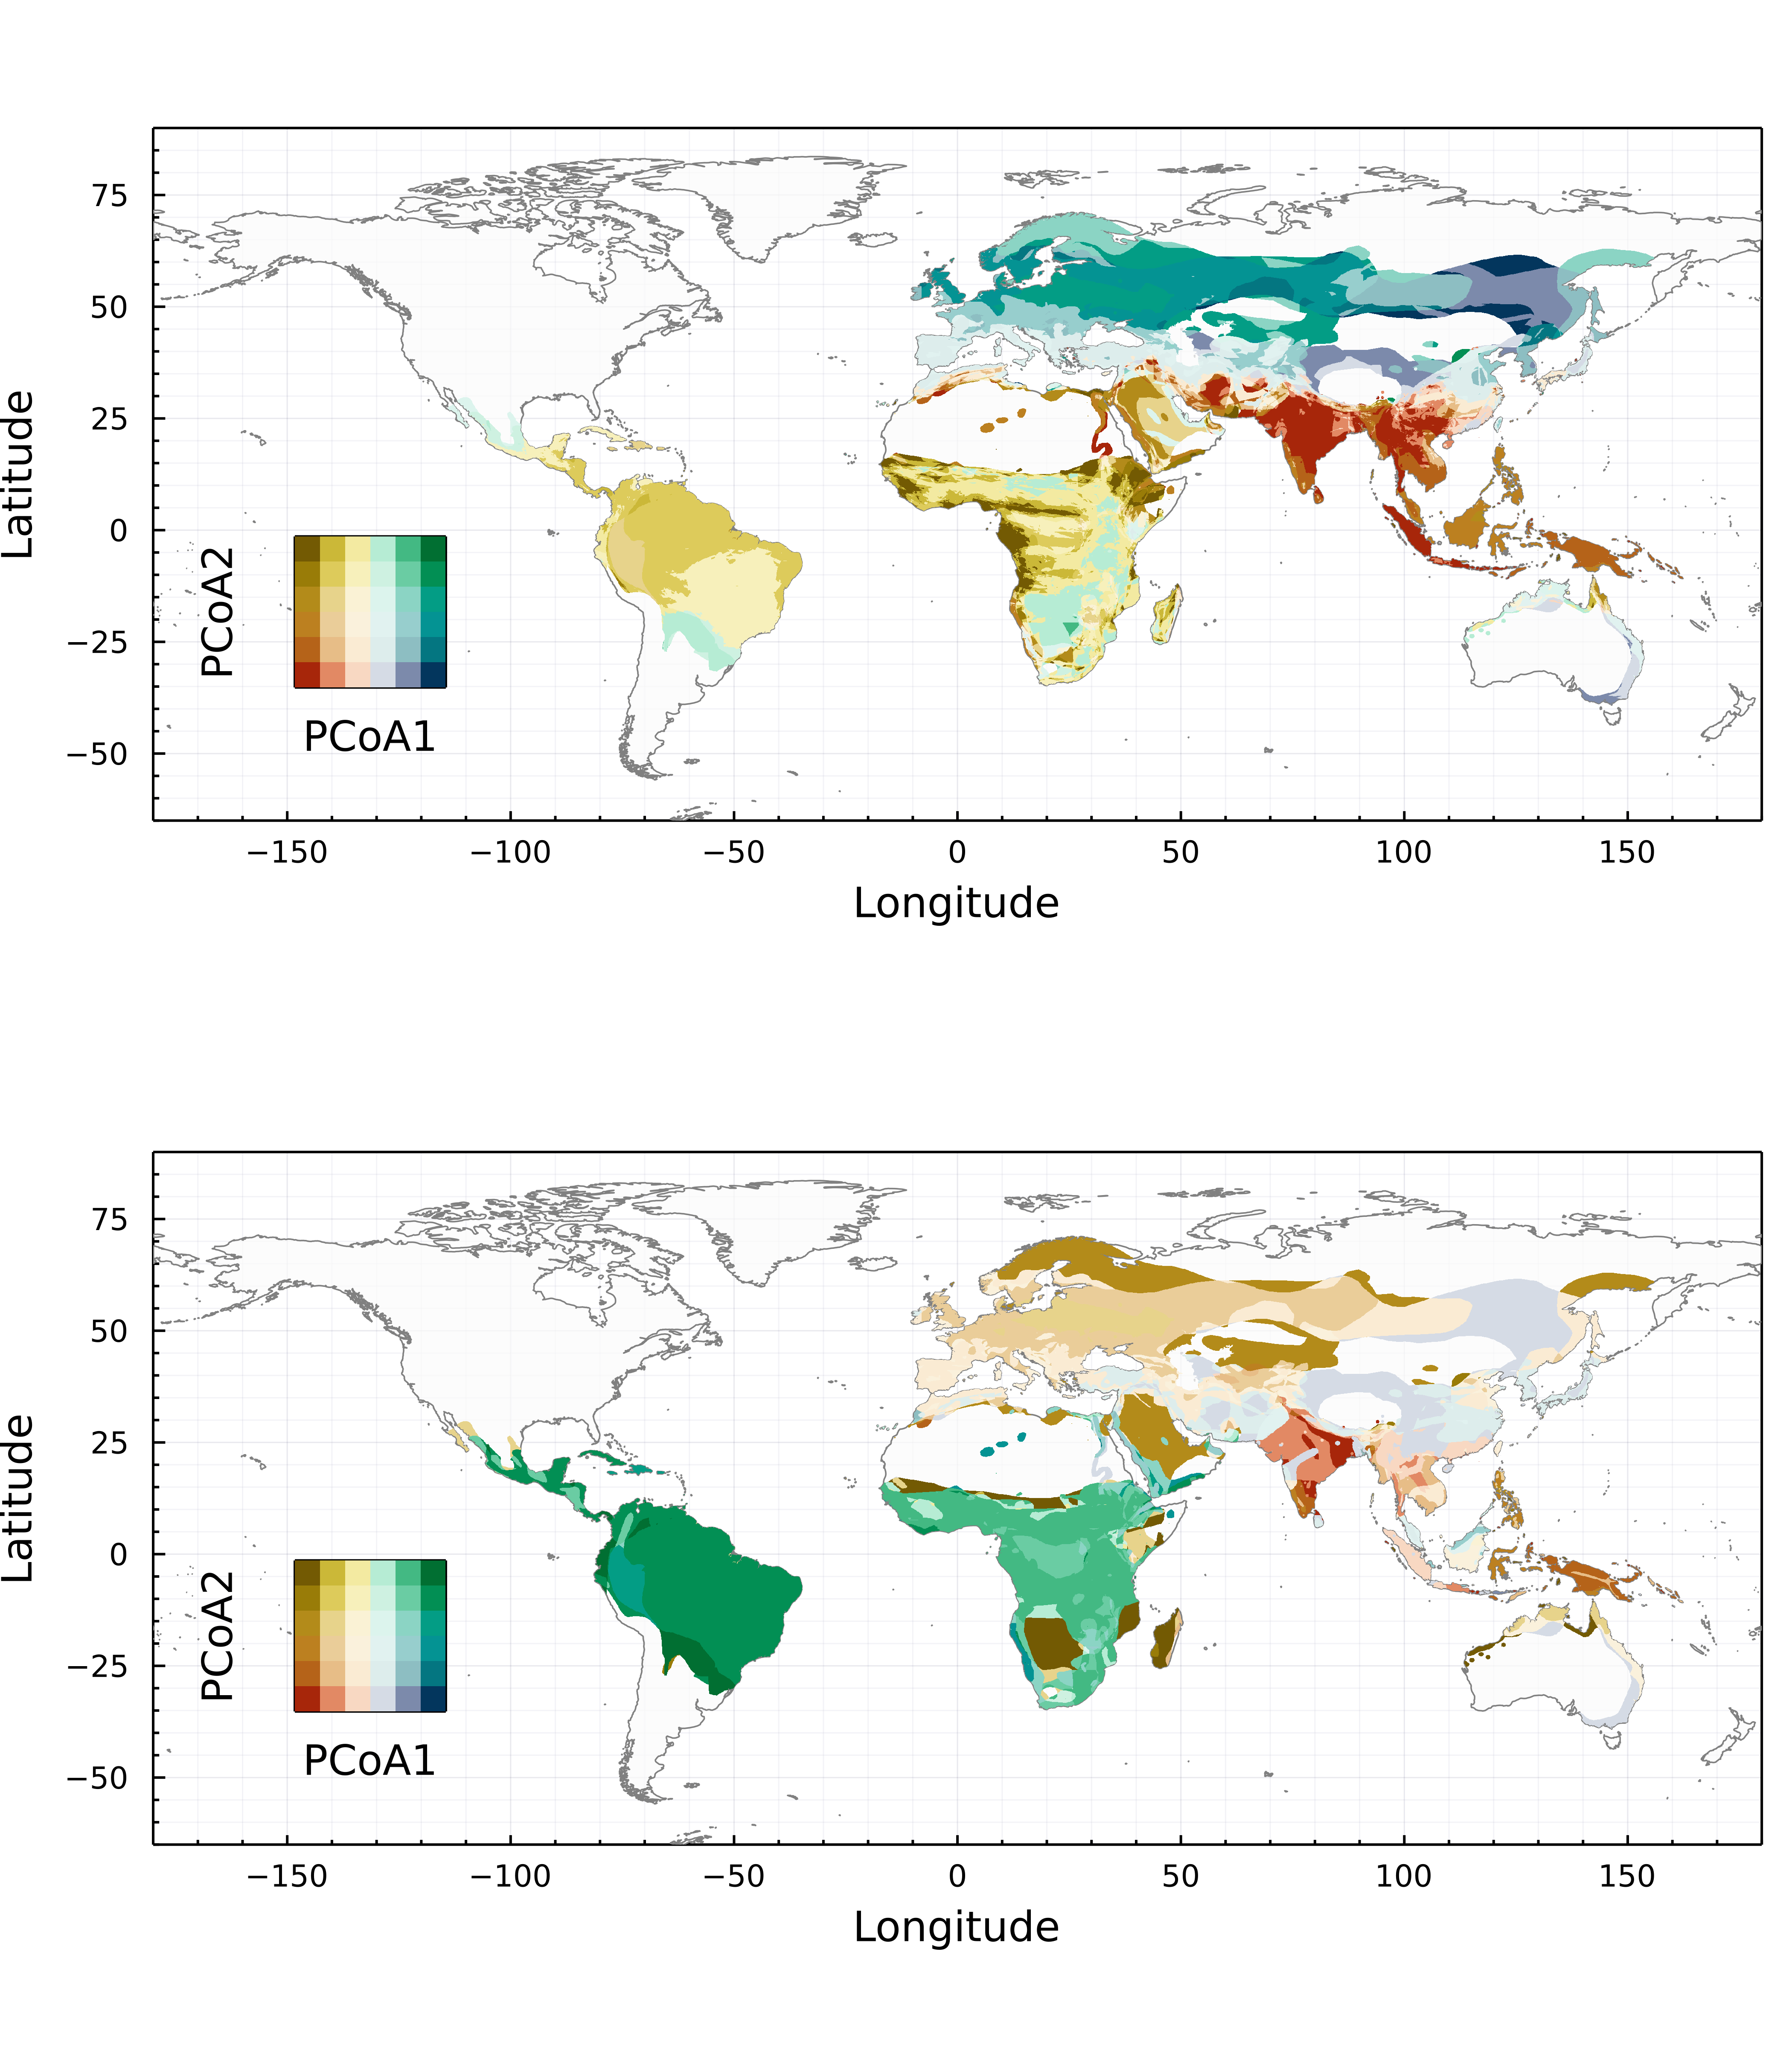
\includegraphics{figures/combined_biogeo.png}
\caption{\textbf{Bat and betacoronavirus biogeographic regions.}
Phylogeography of bats (top) and viruses (bottom) is categorized based
on analysis of bat distributions paired with bat or virus phylogeny. The
different colors show tendencies to separate alongside the first two
components of a PCoA. Note that the PCoA for the bats and viruses are
independent, and so cannot be compared directly -- that being said, the
regions can be compared across maps.}\label{fig:biogeo}
}
\end{figure}

Overall, these results suggest that the boundaries of bat and
betacoronavirus biogeographic regions are broadly consistent at a global
scale; perfect matching between the biogeographic regions would have
indicated that the signal of virus distribution is fully predicted by
bat hosts ranges. Areas for which the biogeographic regions for bats and
betacoronaviruses differ are primarily (i) southeast Asia and southern
China, and (ii) the Arabian peninsula, which are both regions where
zoonotic transmission has been documented (potentially driving a unique
level of viral sampling effort that generates these patterns). These
spatially limited mismatches nonwithstanding, the large level of
congruence may be surprising, given that cross-species transmission may
play a stronger role in coronavirus diversification than
cospeciation---\textsuperscript{\textbf{Anthony2017GloPat?}}a property
that would theoretically allow for substantial broad divergence in their
biogeography. However, host jumps at the family level or higher are
relatively rare and significant events in coronavirus evolutionary
history;\textsuperscript{\textbf{Anthony2017GloPat?},\textbf{Latinne2020OriCro?}}
as a result, the mosaic of betacoronavirus phylogeography is assembled
from a set of overlapping smaller coevolutionary systems, superimposed
in space and filtered by the importance of different subgroups in local
host communities. For example, the most speciose and cosmopolitan family
of bats, the vesper bats (Vespertilionidae), are considered the primary
hosts of the subgenus \emph{Merbecovirus} (MERS-like
viruses);\textsuperscript{\textbf{Latinne2020OriCro?},\textbf{Ruiz-Aravena2022EcoEvo?}}
but in the Americas, where merbecoviruses are the only lineage present,
they have only been found in other bat taxa (\emph{e.g.}, Molossidae,
Phyllostomidae).\textsuperscript{\textbf{Anthony2013CorBat?},\textbf{Goes2013NovBat?},\textbf{Goes2016GenDiv?},\textbf{Brandao2008CorDet?}}
At the coarsest scale, these heterogeneities are lost, and
betacoronavirus biogeography tracks the deep rifts in bat evolutionary
history---but within broad regions, the component coevolutionary systems
may have very different dynamics.

\hypertarget{hotspots-of-bat-and-betacoronavirus-biodiversity-are-distinct}{%
\subsection{Hotspots of bat and betacoronavirus biodiversity are
distinct}\label{hotspots-of-bat-and-betacoronavirus-biodiversity-are-distinct}}

Bats, the second most diverse groups of mammals, are found worldwide;
gradients in their species richness generally track broader patterns of
mammal diversity,\textsuperscript{\textbf{Tanalgo2022Mapping?}} with a
striking Neotropical hotspot (especially in the Amazon basin) and a
secondary hotspot centered in Indochina. These hotspots of bat diversity
are generally presumed to be hotspots of viral adaptive radiation, and
therefore areas of concern for human
health.\textsuperscript{\textbf{Anthony2017GloPat?},\textbf{Olival2017HosVir?}}
However, the hotspots of known bat betacoronavirus hosts show a distinct
pattern, with primary hotspots (both in terms of area and higher values)
of host richness situated in southeast Asia, parts of southern Europe,
and to a lesser extent parts of Africa in the -25-0 range of latitudes
(fig.~\ref{fig:richness}; top). Although hundreds of species likely host
undiscovered betacoronaviruses, machine learning predictions have
suggested that these undiscovered reservoirs should follow the same
diversity gradient.\textsuperscript{\textbf{Becker2022OptPre?}} In
principle, these hotspots of locally-diverse, virus-rich bat communities
should drive more adaptive diversification in their viruses.

\begin{figure}
\hypertarget{fig:richness}{%
\centering
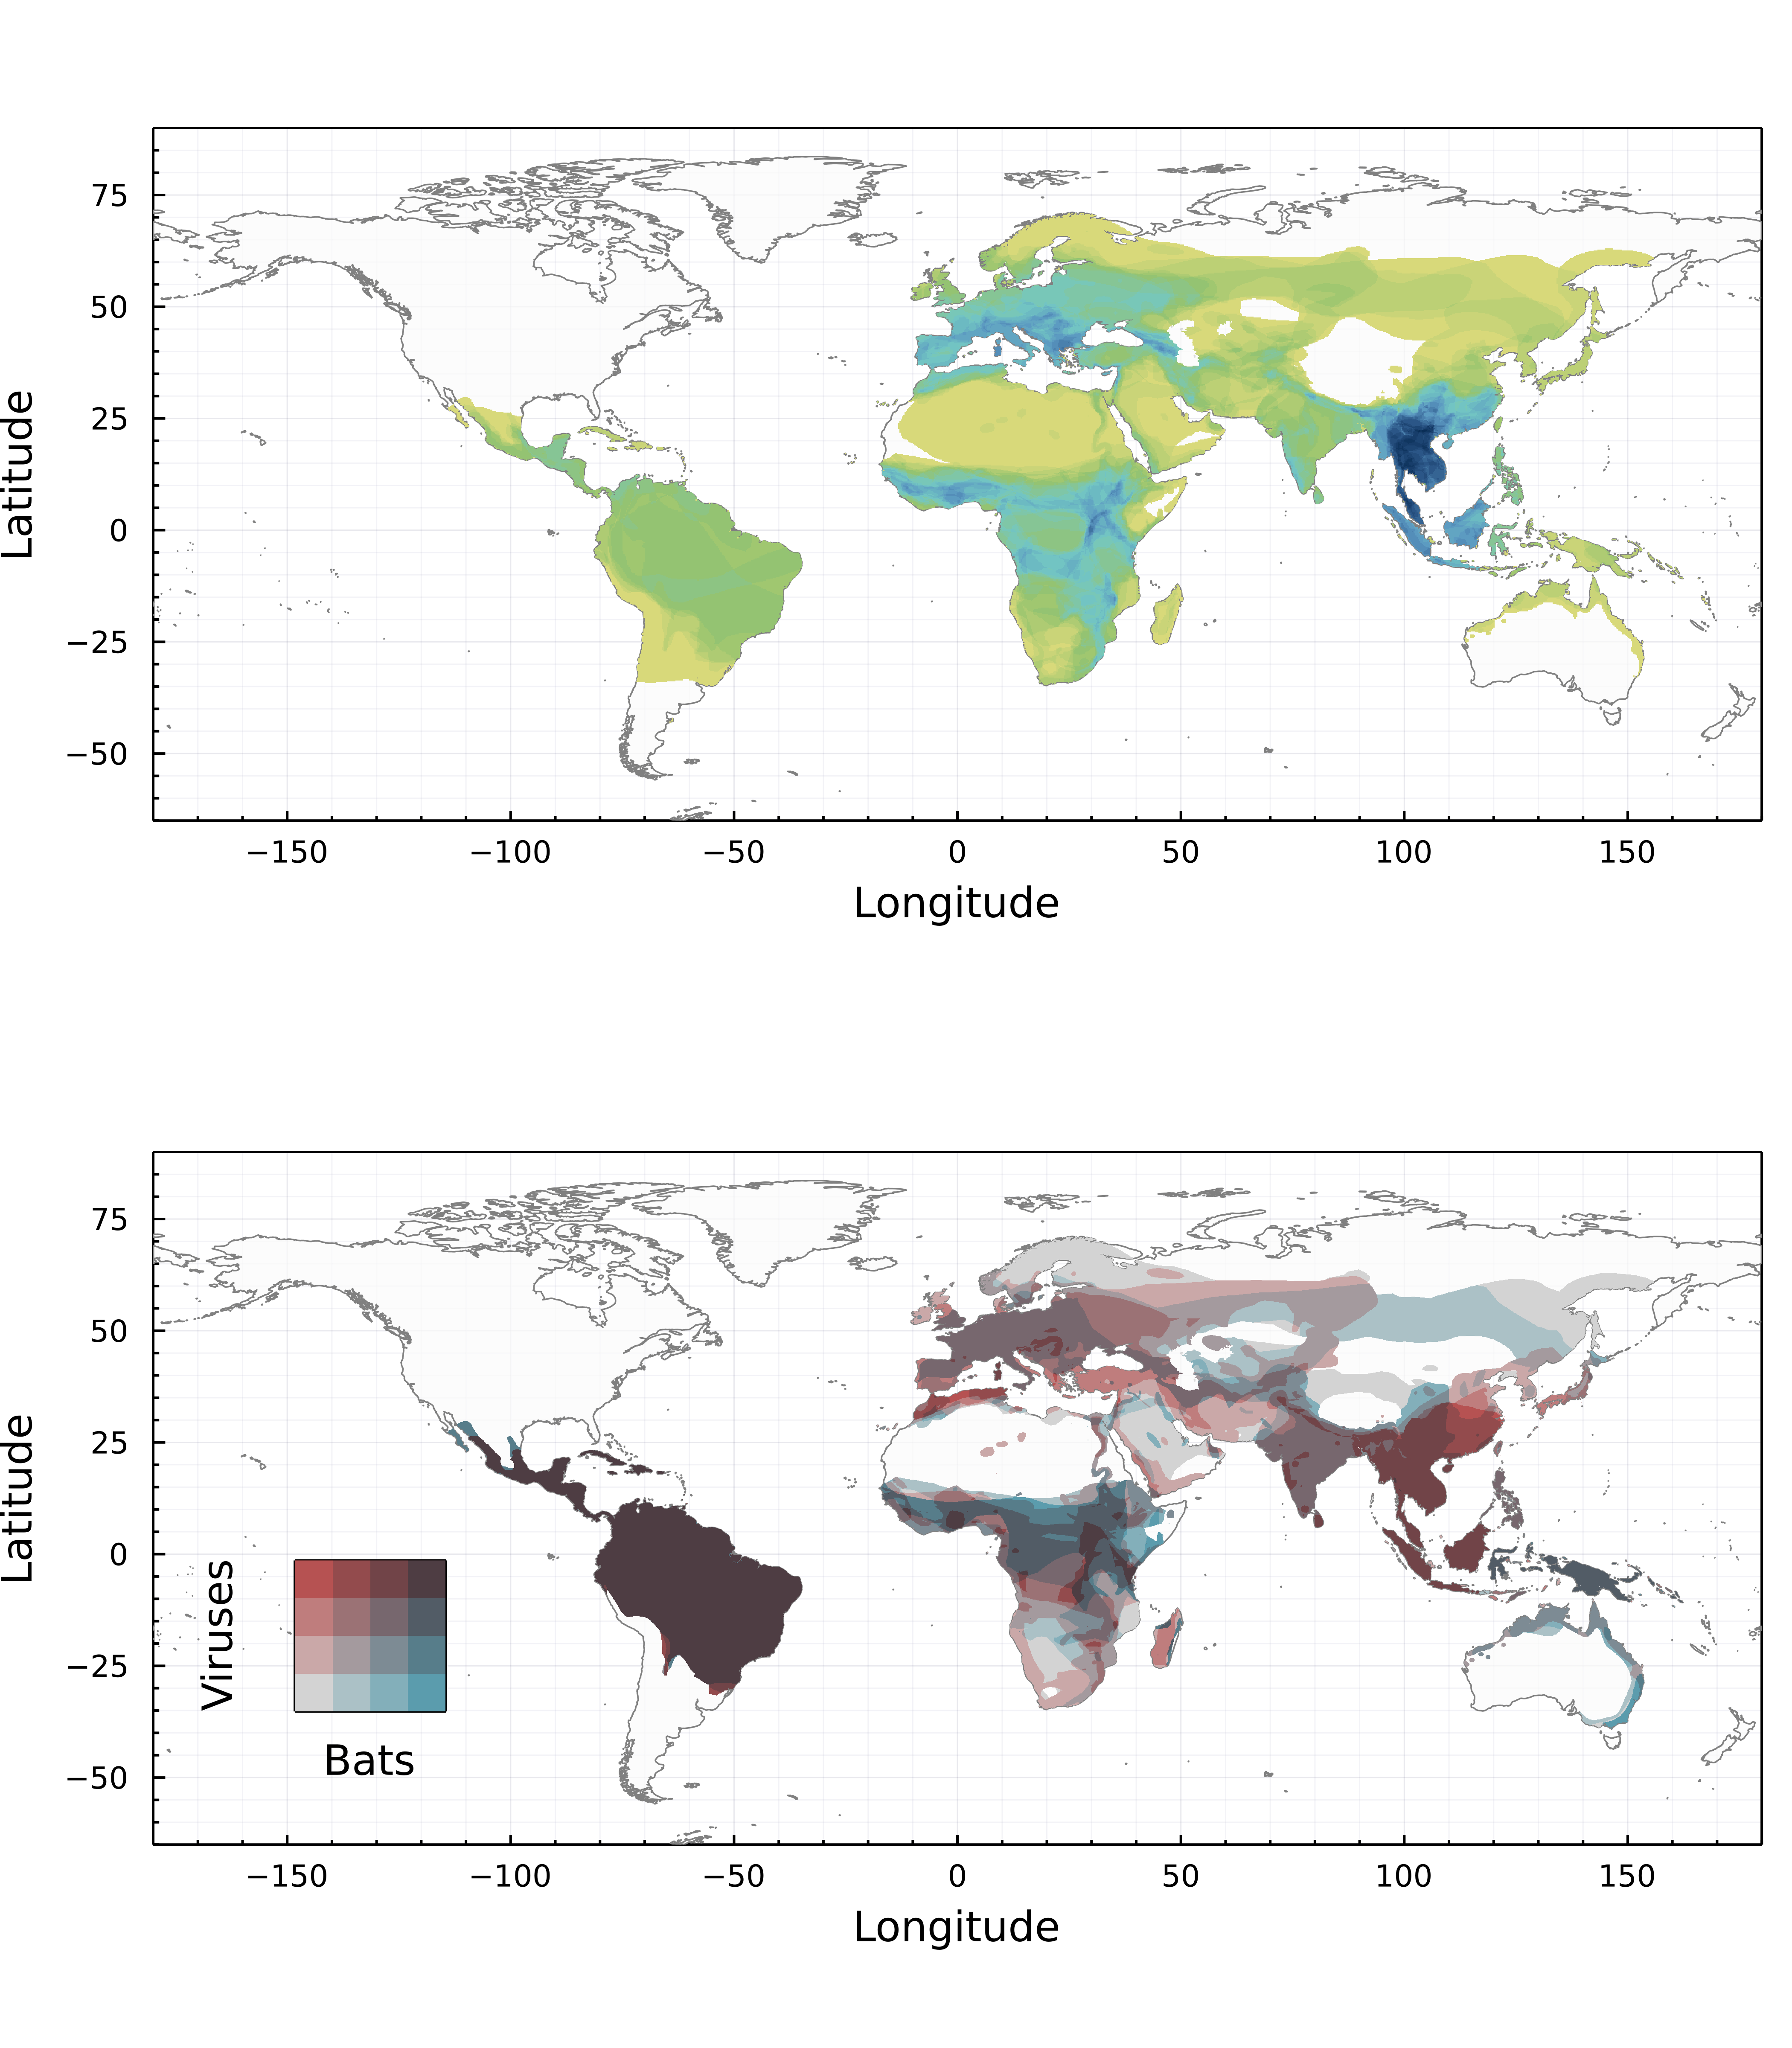
\includegraphics{figures/combined_richness.png}
\caption{\textbf{Bat and betacoronavirus diversity.} Top panel: relative
diversity of known bat hosts of betacoronaviruses. This map shows that
the region with the largest number of possible hosts is South-Eastern
Asia. Bottom panel: congruence between the evolutionary distinctiveness
of the hosts (grey to blue) and the viruses (grey to
red).}\label{fig:richness}
}
\end{figure}

However, we find that the global pattern of betacoronavirus phylogenetic
distinctiveness is quite distinct from both bat host richness and
phylogenetic distinctiveness (fig.~\ref{fig:richness}; bottom). In
contrast to the sparsity of Neotropical betacoronavirus hosts, South and
Central America have the most evolutionary distinct hosts \emph{and}
viruses, followed by secondary hotspots in southeast Asia and the Rift
Valley region have mostly distinct viruses. Some degree of sampling bias
may contribute to these patterns: for example, the Neotropics are one of
the places where the fewest bat betacoronavirus sequences have been
generated,\textsuperscript{\textbf{Worobey2022HuaMar?},\textbf{Temmam2022BatCor?},\textbf{Boni2020EvoOri?}}
resulting in a sparser phylogenetic tree, and artificially inflating
distinctiveness; conversely, disproportionate research effort in eastern
China\textsuperscript{\textbf{Cohen2022SamStr?}} may have led to a more
complete inventory of the local diversity of coronaviruses, again
inflating these metrics relative to underlying patterns. Even accounting
for these potential biases, though, there is obvious heterogeneity in
betacoronavirus evolutionary distinctiveness that is distinct from
overall bat diversity.

Overall, these patterns recapitulate the evolutionary history of both
the order Chiroptera and the genus \emph{Betacoronavirus}. Horseshoe
bats (Rhinolophidae) include the reservoirs of the SARS-like viruses
(subgenus \emph{Sarbecovirus}), the group of pandemic threats that have
been of the greatest interest to
researchers\textsuperscript{\textbf{Latinne2020OriCro?}} (and so have
been sampled most
intensively).\textsuperscript{\textbf{Cohen2022SamStr?}} The hotspots of
host richness and viral diversity in southeast Asia---both of which are
disproportionately high, considering the global landscape of bat species
richness---are almost entirely driven by viral adaptive radiation
through host switching within this
clade\textsuperscript{\textbf{Becker2022OptPre?},\textbf{Ruiz-Aravena2022EcoEvo?}}.
In contrast, the Neotropical hotspot of viral distinctiveness is driven
by isolation by host vicariance. Out of the four main groups of
betacoronaviruses, only merbecoviruses have been found in animals in the
Americas--- an introduction that is generally presumed to be
ancient.\textsuperscript{\textbf{Ruiz-Aravena2022EcoEvo?},\textbf{Olival2020PosRev?}}
While comparatively understudied, New World merbecoviruses have been
found in the ghost-faced bats (Mormoopidae), Neotropical leaf-nosed bats
(Phyllostomidae), and free-tailed bats
(Molossidae).\textsuperscript{\textbf{Anthony2013CorBat?},\textbf{Goes2013NovBat?},\textbf{Goes2016GenDiv?},\textbf{Brandao2008CorDet?}}
The former two groups and a clade of the latter are endemic to the
Neotropics, while the explosive adaptive radiations of the phyllostomids
are responsible for the hotspot of bat diversity in the
Amazon.\textsuperscript{\textbf{Ammerman2012FirMol?}} Together, these
clades of New World bats play host to a distinct regime of
betacoronavirus coevolution.

Our approach is potentially limited by sampling bias: key hotspots
identified by our model have, indeed, been sampled intensely following
major zoonotic emergence events. In these areas, more betacoronavirus
hosts will have been discovered, leading to higher overall diversity and
potentially higher sharing. Similarly, hotspots of evolutionary
uniqueness - as in the Arabian peninsula - could reflect much broader
lineages that have only been sampled in focal areas for public health.
While the discovery of new branches of bat-betacoronavirus coevolution
is certainly likely, and might change some of the observed patterns, our
framework is likely to be fairly robust: the 126 hosts in our study
capture nearly 10\% of global bat diversity, and the underlying
evolutionary patterns they represent are much less sensitive to new
information than any inferences about viral evolution.

\hypertarget{coevolutionary-regimes-structure-evolutionary-potential-for-zoonotic-emergence}{%
\subsection{Coevolutionary regimes structure evolutionary potential for
zoonotic
emergence}\label{coevolutionary-regimes-structure-evolutionary-potential-for-zoonotic-emergence}}

The existence of well-defined cophylogenetic regions suggests that the
bat-betacoronavirus system is spatially fragmented enough to create
divergent coevolutionary trajectories; in turn, this coevolutionary
mosaic may alter the risk of zoonotic emergence. These ideas are,
respectively, supported by the existence of hotspots of viral uniqueness
and the diverse origins of human betacoronaviruses. Together, this
framework points to a predictable relationship between host community
structure and coevolutionary pressure: phylogeographic structure in bat
hosts (and their diverse immune
strategies)\textsuperscript{\textbf{Banerjee2020NovIns?}} creates a
landscape of selective pressure; the trajectory of viruses'
coevolutionary response is, in turn, constrained by their opportunities
for either specialization or diversification through host jumps and
recombination.

Based on the geographic mosaic theory of coevolution, we developed a
trivariate map of coevolutionary pressure (fig.~\ref{fig:trivariate}):
(1) \emph{host phylogenetic diversity}: a high diversity of evolutionary
histories should expose viruses to more variation in host immune traits;
(2) \emph{host community uniqueness}: exposure to greater host trait
heterogeneity can drive viral diversification, and coevolving with more
unique host communities should create more unique branches of viral
evolution; and (3) propensity for \emph{viral sharing}: frequent
cross-species transmission may act as a buffer on selective pressure,
while lower rates of exchange may enable more simultaneous trajectories
of viral specialization to coexist within a given community. We combine
global maps of all three to generate a map of coevolutionary regimes,
where close colors represent similar risks, and paler pixels represent
overall higher risk (see Methods). We find that these regions do not
neatly overlap with those defined in fig.~\ref{fig:biogeo} or
fig.~\ref{fig:richness}, reinforcing the notion that local-scale
coevolutionary mosaics can form within cophylogenetic regions.

\begin{figure}
\hypertarget{fig:trivariate}{%
\centering
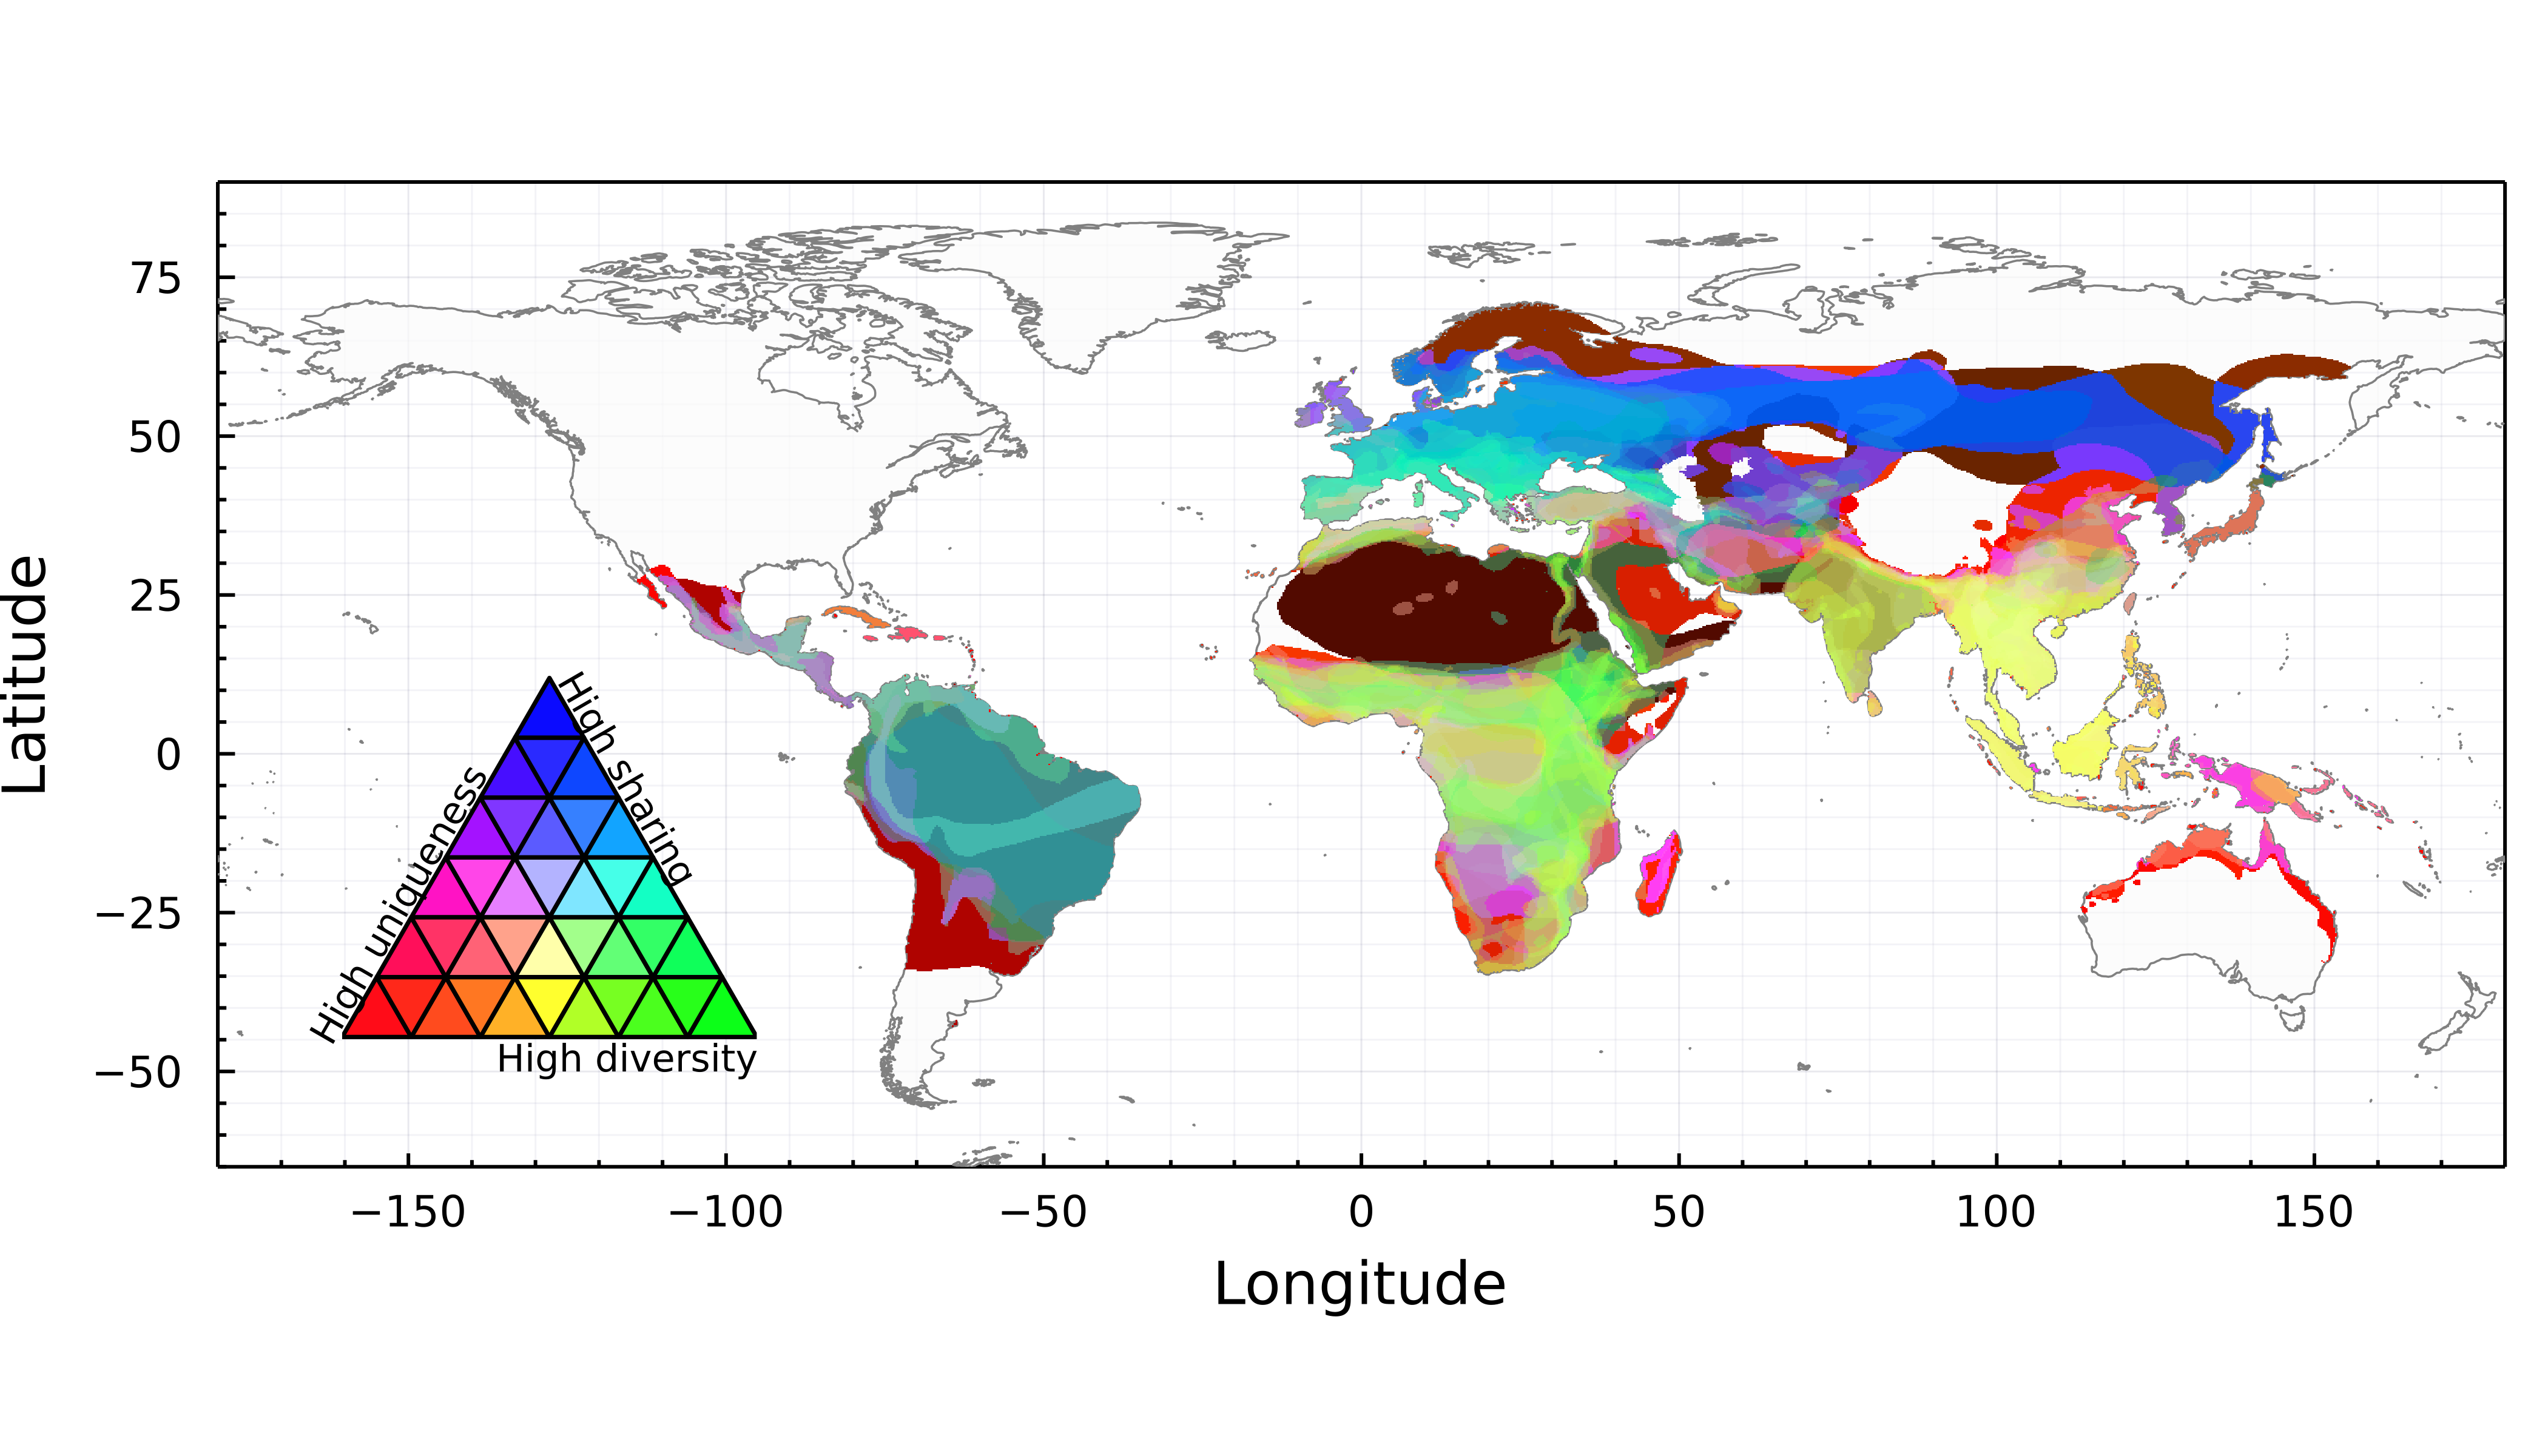
\includegraphics{figures/risk_trivariate.png}
\caption{\textbf{Trivariate additive mapping of the components of risk.}
Viral sharing runs from yellow (low) to blue (high); host phylogenetic
diversity runs from pink (low) to high (green); and host compositional
uniqueness runs from cyan (low) to red (high). The GMTC suggests that
the highest evolutionary potential for emergence exists in unique and
diverse host communities with low viral sharing, \emph{i.e.} pixels
around yellow. All components within bat host ranges are scaled in
brightness so that a pixel with no sharing, no phylogenetic diversity,
and no compositional uniqueness would be black, and a pixel with maximal
values for each would be white.}\label{fig:trivariate}
}
\end{figure}

The greatest evolutionary potential for zoonotic emergence exists where
pathogen pools have a high genetic diversity and high propensity for
cross-species transmission. In our framework, emergence risk is
therefore maximized under higher phylogenetic diversity (viruses are
exposed to different host clades), higher host uniqueness (viruses are
experiencing novel, heterogeneous host traits combinations), and low to
medium viral sharing (host-virus pairs can coevolve independently, but
divergent viruses may still have opportunities for recombination). In
fig.~\ref{fig:trivariate}, this corresponds to yellow areas (dynamics
dominated by low viral sharing, with equal contributions of selection
mosaics and trait remixing; southeast Asia, and the Indian
sub-continent), green-yellow areas (dynamics with low viral sharing but
dominated by the selection mosaic effect of host diversity; sub-Saharan
Africa), and red-yellow areas (dynamics with low viral sharing but
dominated by trait remixing in host communities; the Middle East).
Translating this axis of variation back into a univariate risk map
(fig.~\ref{fig:risk}) highlights that this evolutionary landscape has a
striking correspondence to regions where zoonotic betacoronaviruses have
previously emerged. Our findings align with predictions regarding the
spatial location of cross-species transmission. These locations not only
pose a potential risk of viral jumps that could endanger human health
but also provide valuable information for monitoring wildlife health.
This could guide us to determine where and what measures to implement
for effectively monitoring wildlife and human betacoronavirus outbreaks
before they escalate to critical levels. Nevertheless, there are
actually very few documented cases of emergence events, and similarities
could be some degree of coincidental.

Compared to approaches that map emergence risk based only on the number
of known bat hosts of betacoronaviruses, our framework suggests regions
where high viral sharing dominates coevolutionary dynamics---such as
Latin America, or Eurasia above a northing of 30---would pose less of a
relative risk of zoonotic emergence. Nevertheless, areas of high host
uniqueness coupled with high viral sharing (red-to-pink in
fig.~\ref{fig:trivariate}) could create hotspots facilitated by viral
codivergence. Our framework identifies Madagascar, where most bat
species are endemic following evolutionary divergence from sister
species in both African and Asian
continents,\textsuperscript{\textbf{Shi2014DeeDiv?}} as one such
hotspot; interestingly, a recent
study\textsuperscript{\textbf{Kettenburg2022FulGen?}} reported a novel
and highly divergent lineage of nobecoviruses from Madagascar-endemic
pteropid bat species (\emph{Pteropus rufus} and \emph{Rousettus
madagascariensis}), again supporting the predictive power of the
coevolutionary framework.

\begin{figure}
\hypertarget{fig:risk}{%
\centering
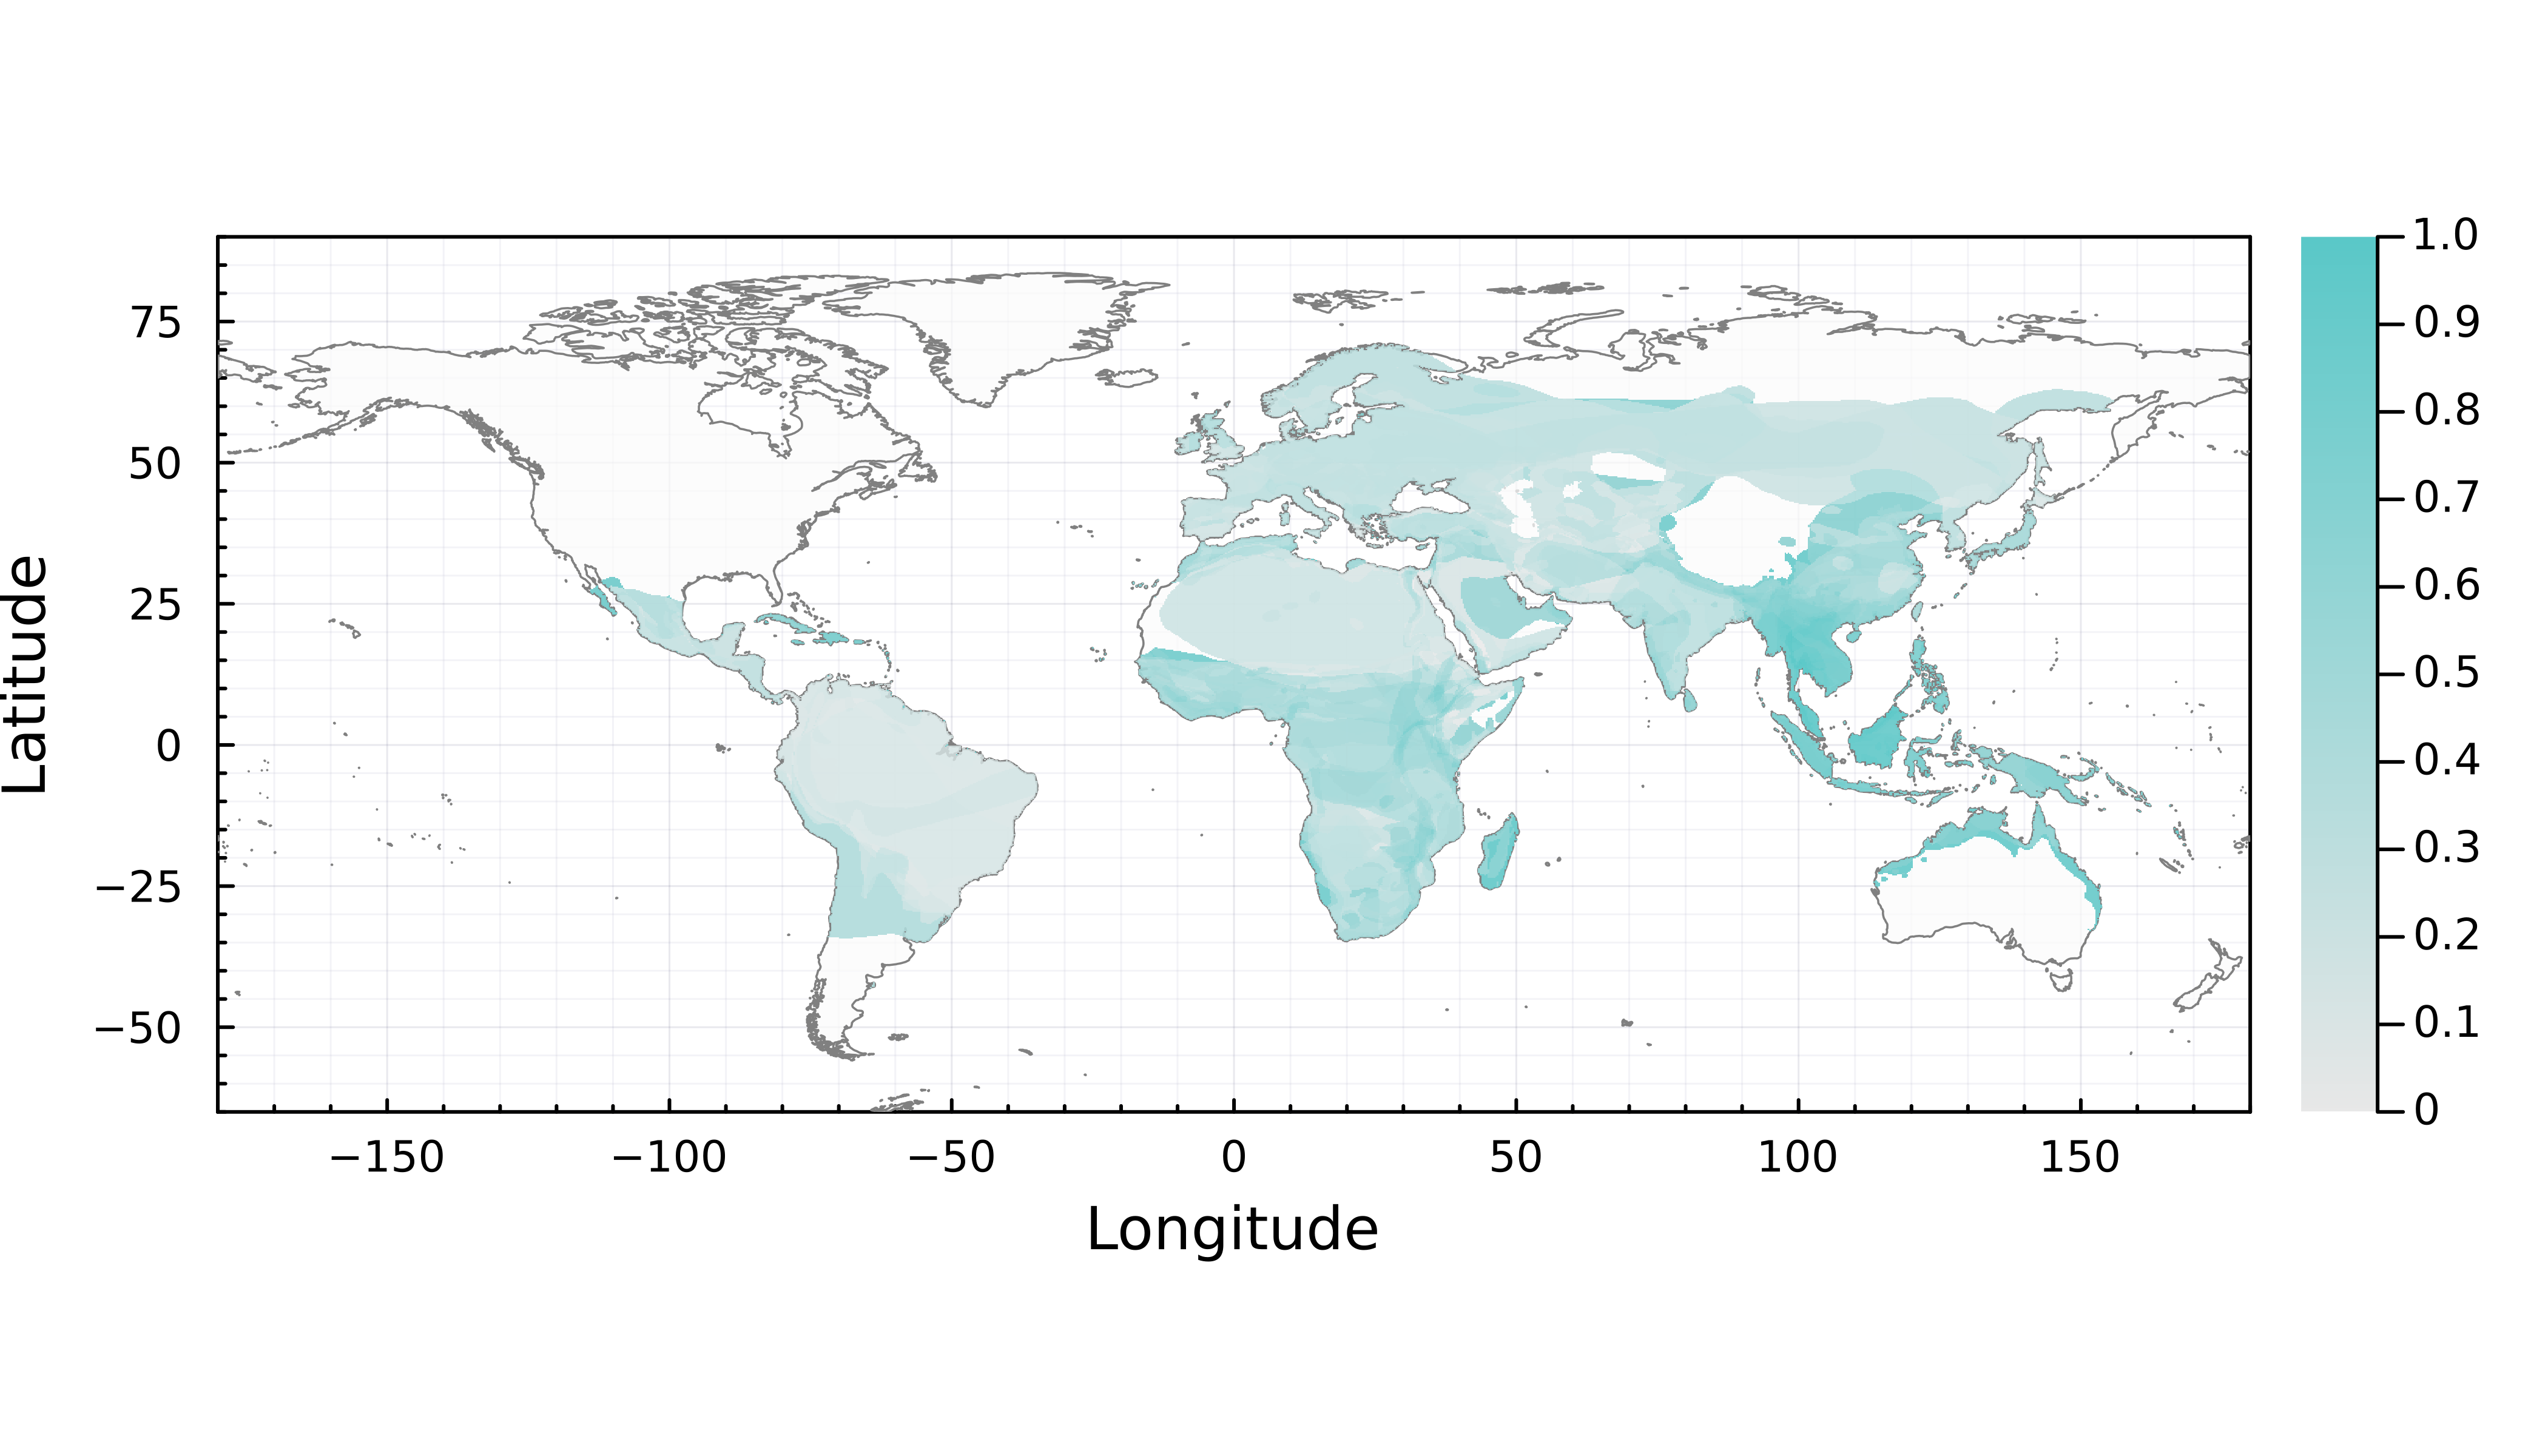
\includegraphics{figures/risk_map.png}
\caption{\textbf{Evolutionary potential for zoonotic emergence of
bat-origin betacoronaviruses.} Risk is a composite measure of the color
value and angular distance to the yellow hue in
fig.~\ref{fig:trivariate} (see Methods).}\label{fig:risk}
}
\end{figure}

\hypertarget{human-landscapes-filter-the-geography-of-emergence-risk}{%
\subsection{Human landscapes filter the geography of emergence
risk}\label{human-landscapes-filter-the-geography-of-emergence-risk}}

The relationship between the underlying pathogen pool and emergence risk
is mediated by both human-wildlife interfaces (the probability of
spillover) and opportunities for onward horizontal transmission (the
probability that spillovers become
epidemics)\textsuperscript{\textbf{Plowright2017PatZoo?}}. It must be
noted that the assesment of risk based on the GMTC mechanisms does not
account for human presence; for this reason, it represents ``potential''
level of risk, which must be re-evaluated in the light of human
presence. As a proxy for both, we finally overlaid the risk component
from the composite map (see above) with the proportion of built land, as
a proxy for a mix of habitat disturbance, potential for bat synanthropy
or contact with bridge hosts like
livestock,\textsuperscript{\textbf{Rulli2021LanCha?},\textbf{Cui2019OriEvo?}}
and human population density and
connectivity\textsuperscript{\textbf{Plowright2017PatZoo?},\textbf{Muylaert2022PreFut?},\textbf{Hassell2017UrbDis?}}
(fig.~\ref{fig:compound}). Accounting for these factors, most of South
America and Europe are at comparatively lower risk, as--although densely
populated--settlements tend to be in areas with lower potential risk.
Conversely, regions like Malaysia and the northern coast of Australia
have a high evolutionary risk component, but should represent a
relatively lower effective risk due to low human density. However,
southeast Asia, the Indian subcontinent, and scattered hotspots in
sub-Saharan Africa are at high risk due to the overlap between human
populations and natural opportunities for cross-species transmission of
betacoronaviruses.

\begin{figure}
\hypertarget{fig:compound}{%
\centering
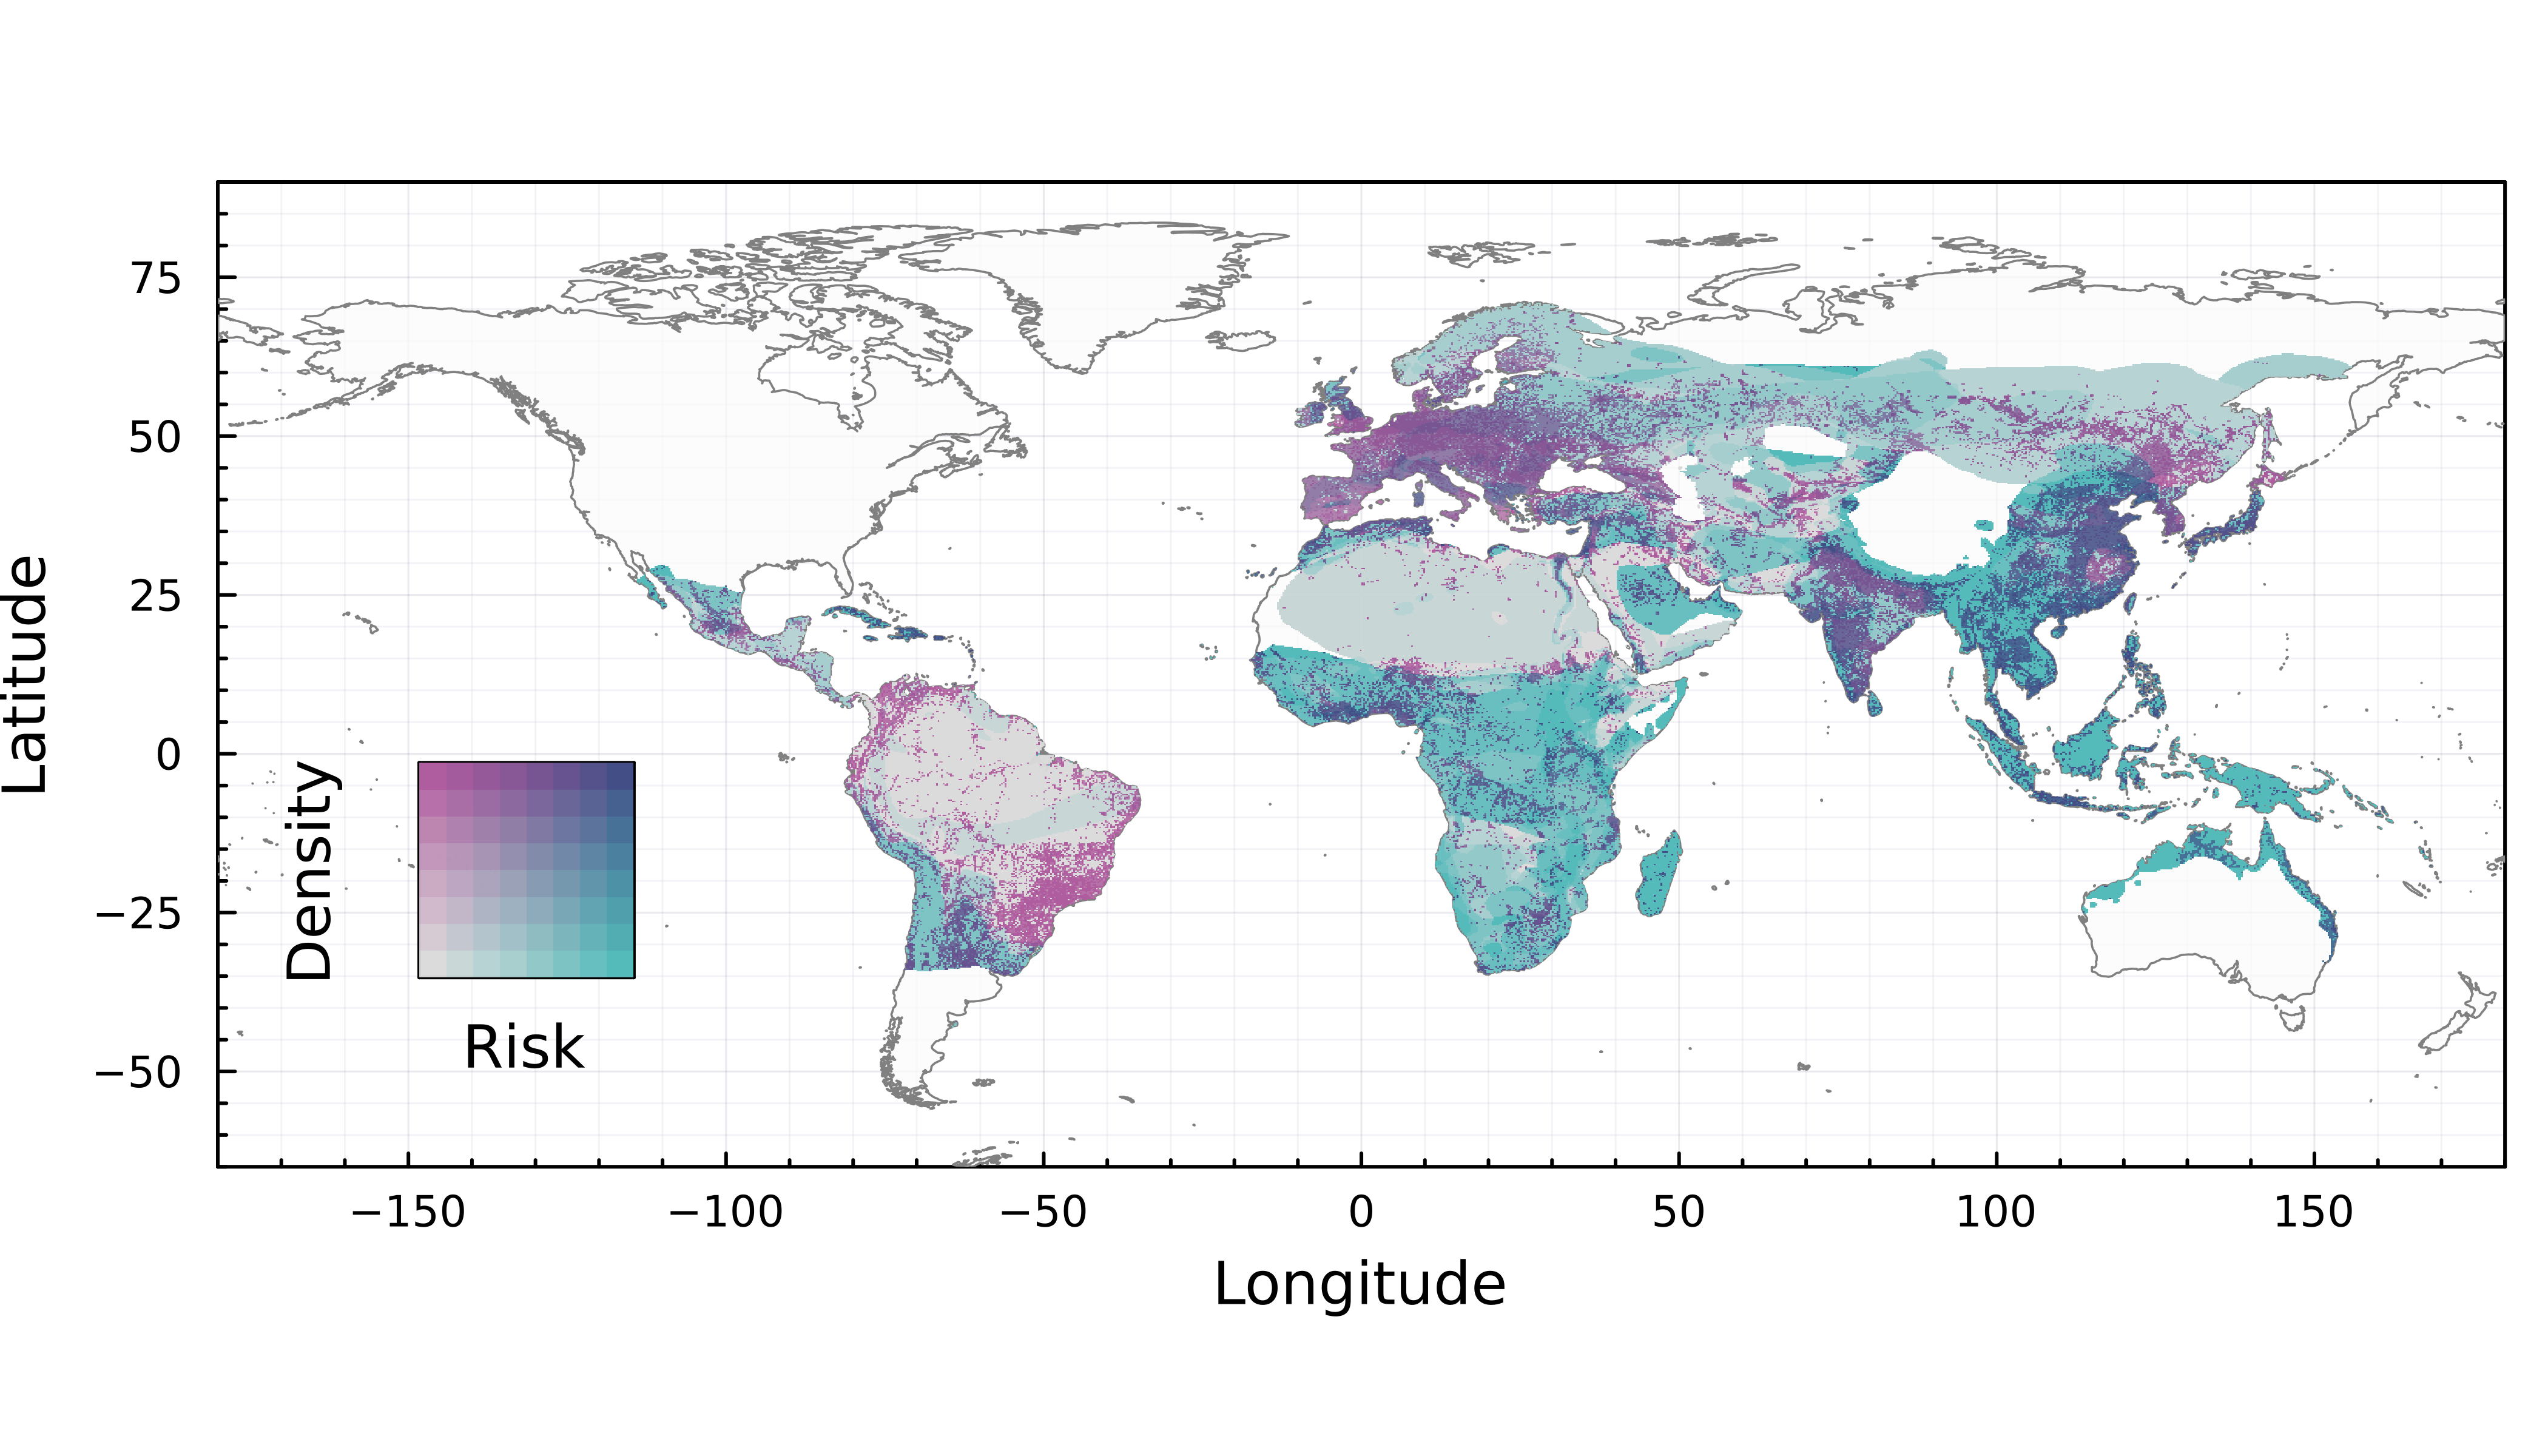
\includegraphics{figures/risk_compounded.png}
\caption{\textbf{Overlap between evolutionary potential and ecological
opportunity for zoonotic emergence.} Overlap of the percent of each
pixel occupied by urbanized structures, representing the degree of
settlement, on the spillover risk map (where the risk comes only from
wildlife, and ignores multi-hosts chains of transmissions including
non-bats hosts). Darker pixels correspond to more risk, in that the
GMTC-derived risk of fig.~\ref{fig:risk} is high \emph{and} the pixel is
densely occupied by human populations.}\label{fig:compound}
}
\end{figure}

Reassuringly, these predictions correspond to the geographic origins of
the three bat-origin coronaviruses that have recently emerged in human
populations. While available information puts the spillover of
SARS-CoV-2 in a live animal market in Wuhan, China, the ultimate origin
of the virus is almost certainly in a divergent lineage of
sarbecoviruses from Indochina that was poorly characterized prior to the
pandemic.\textsuperscript{\textbf{Worobey2022HuaMar?},\textbf{Temmam2022BatCor?},\textbf{Boni2020EvoOri?}}
Similarly, the SARS-CoV outbreak began in Guangdong province in 2002,
reaching humans through small carnivore bridge hosts, but was eventually
traced back to a set of likely progenitor viruses found in cave-dwelling
horseshoe bats in Yunnan
province;\textsuperscript{\textbf{Hu2017DisRic?}} nearby, antibody
evidence has indicated human exposure to SARS-like
viruses.\textsuperscript{\textbf{Wang2018SerEvi?}} MERS-CoV was first
detected in Jordan, but is widespread in camels in East Africa and the
Middle East, and may have reached its bridge host decades earlier than
originally supposed;\textsuperscript{\textbf{Muller2014MerCor?}} as a
result, the geography of the original bat-to-camel transmission is still
widely regarded as uncertain. All of these are broadly consistent with
the risk factors we identify. Notably, India and west Africa are
additional hotspots that have yet to experience the emergence of a bat
coronavirus into human populations, but may still be at
risk---particularly given known gaps in bat
surveillance,\textsuperscript{\textbf{Cohen2022SamStr?}} and a dense
population in both regions with global connectivity. In any of these
regions, surveillance on viral reservoirs can be paired with targeted
monitoring of high-risk human populations (i.e., those with regular
wildlife contact)\textsuperscript{\textbf{Xu2004EpiClu?}} for maximum
impact.

\hypertarget{conclusion}{%
\section{Conclusion}\label{conclusion}}

Bats emerged around 64 million years ago, and are one of the most
diverse mammalian orders, with more than 1,400 estimated
species.\textsuperscript{\textbf{Peixoto2018SynEco?},\textbf{Simmons2020BatSpe?}}
They exhibit a broad variety of habitat use, behaviour, and feeding
strategies, putting them at key positions in the delivery and
provisioning of several ecosystem services, tied to important
ecosystem-derived benefits to
humans.\textsuperscript{\textbf{Kasso2013EcoEco?}} Over two-thirds of
bats are known to be either obligate or facultative insectivores,
therefore actively contributing for agricultural pest
control,\textsuperscript{\textbf{Voigt2016BatAnt?},\textbf{Williams-Guillen2008BatLim?}}
and vectors of pathogens that put a risk on human
health;\textsuperscript{\textbf{Gonsalves2013MosCon?},\textbf{Gonsalves2013MosInf?}}
some other species are essential links in many seed-dispersal
networks.\textsuperscript{\textbf{Mello2011MisPar?}} However, many of
these species face a high risk of extinction, particularly given
persecution and killings that sometimes follows from messaging about
their role in disease emergence. Areas where bats, viruses, and humans
co-occur are not always hotspots of risk for human heath; as such,
developing more precise ways to map zoonotic hazards can help bats and
humans coexist safely, and support the conservation of these important
and unique animals.

Here, we propose a simple framework with broad explanatory power that
helps contextualize discoveries like highly divergent nobecoviruses in
Madagascar and the once-neglected adaptive radiation of sarbecoviruses
in the Indochinese peninsula. In doing so, it advances ecological theory
beyond the current state of the art for global maps of emergence risk.
For example, previous studies that have used host richness as a proxy
have predicted a high diversity of unsampled bat
viruses,\textsuperscript{\textbf{Olival2017HosVir?}} bat
coronaviruses,\textsuperscript{\textbf{Anthony2017GloPat?}} and even
specifically
betacoronaviruses\textsuperscript{\textbf{Becker2022OptPre?}} in both
the Amazon and southeast Asia. While we find that both regions are
characterized by unique and diverse communities of both hosts and
viruses, our framework is able to identify key differences between the
two systems. We find that the merbecovirus complex in Latin America has
been a unique branch of evolution separate from the rest of the global
pool, but with limited potential for viral diversification--- a finding
that is supported by previous work indicating a higher rate of
codivergence in Latin
America.\textsuperscript{\textbf{Anthony2017GloPat?},\textbf{Caraballo2022CroTra?}}
In contrast, in southeast Asia, host richness and viral distinctiveness
are high but sharing is low; this suggests a different type of
evolutionary dynamics that could generate high local diversity of
viruses through host switching and viral recombination (see
\emph{e.g.},\textsuperscript{\textbf{Latinne2020OriCro?}} as well as the
discovery of recombinant viruses with genetic material from both the
SARS-CoV and SARS-CoV-2 branches of the Sarbecovirus
lineage).\textsuperscript{\textbf{Wu2021ComSur?}}Both of these regions
are priority areas for sampling, especially given predictions that they
contain many bat hosts of undiscovered
betacoronaviruses.\textsuperscript{\textbf{Becker2022OptPre?},\textbf{Cohen2022SamStr?}}
However, both the evolutionary and ecological aspects of emergence risk
are higher in southeast Asia---a fact that will only become more
relevant, as bats track shifting climates and exchange viruses with
other species, creating a hotspot of elevated cross-species transmission
unique to the
region.\textsuperscript{\textbf{Carlson2022CliCha?},\textbf{Muylaert2022PreFut?}}

Our trivariate additive mapping of components of risk
(fig.~\ref{fig:trivariate}) aims to elicit the complexity of spatial
cross-species transmission risk beyond the mere presence or absence of
the pathogen host in a specific location. By considering coevolutionary
factors such as viral sharing and host uniqueness, we suggest insights
that can aid in identifying potential locations for surveillance of
betacoronavirus circulation and assessing the risk of cross-species
transmission to other mammals. In communities characterized by diverse
but unique host populations, with limited viral sharing between them, we
could encounter viruses that specialize in targeting the immune system
of specific hosts. This implies a low likelihood of infecting novel
hosts but, once locally introduced into a new host (either a new
species, or an immunologically naïve population), the specialized virus
could spread relatively easily due to encountering little immune
resistance (CITE PLOWRIGHT). With the right combination of viral traits,
such as low disease-induced mortality or high transmission rate, this
could lead to successfully spread within the new host community.
However, while high adaptation to a specific host can be advantageous,
it may also lead to maladaptation when the pathogen encounters a new
unsuitable host, potentially resulting in its extinction.

\begin{quote}
Plowright RK, Foley P, Field HE, Dobson AP, Foley JE, Eby P, Daszak P.
Urban habituation, ecological connectivity and epidemic dampening: the
emergence of Hendra virus from flying foxes (Pteropus spp.). Proceedings
of the Royal Society B: Biological Sciences. 2011 Dec
22;278(1725):3703-12.
\end{quote}

Bats---and the spillover of their viruses---are also sensitive to
anthropogenic factors others than climate change, including
deforestation and other kinds of habitat loss, increased stress, and
greater contact with potential bridge hosts like domesticated
species.\textsuperscript{\textbf{Alves2018GeoVar?},\textbf{Treitler2016EffLoc?},\textbf{Rulli2021LanCha?},\textbf{Mendenhall2014PreBio?}}
This represents a challenge for both conservation strategies and
pandemic prevention,\textsuperscript{\textbf{Amman2011InvRol?}} but
identifying areas at risk, and protecting the health of bats and
ecosystems within those zones, can be a win-win intervention for
both.\textsuperscript{\textbf{Hopkins2021HowIde?},\textbf{Plowright2021LanUse?},\textbf{OHHLEP2022OneHea?}}
As we scale these predictions down in space to finer spatial resolutions
to guide public health actions,\textsuperscript{1} the incorporation of
human activity predictors will become more
importyant.\textsuperscript{2}

\textbf{Acknowledgements}: We acknowledge that this study was conducted
on land within the traditional unceded territory of the Saint Lawrence
Iroquoian, Anishinabewaki, Mohawk, Huron-Wendat, and Omàmiwininiwak
nations. This work was supported by funding to the Viral Emergence
Research Initiative (VERENA) consortium including NSF BII 2021909 and a
grant from Institut de Valorisation des Données (IVADO). This research
was enabled in part by support provided by Calcul Québec
(www.calculquebec.ca) and Compute Canada (www.computecanada.ca). NF is
funded by the NSERC BIOS² CREATE program. TP and NF are funded by the
Courtois Foundation. RLM was supported by Bryce Carmine and Anne Carmine
(née Percival), through the Massey University Foundation. DJB was
supported by the National Institute of General Medical Sciences of the
National Institutes of Health (P20GM134973).

\newpage

\hypertarget{methods}{%
\section{Methods}\label{methods}}

\hypertarget{known-betacoronavirus-hosts}{%
\subsection{\texorpdfstring{Known \emph{Betacoronavirus}
hosts}{Known Betacoronavirus hosts}}\label{known-betacoronavirus-hosts}}

We downloaded the data on bats hosts of \emph{Betacoronavirus} from
\texttt{https://www.viralemergence.org/betacov} on
Apr.~2022,\textsuperscript{\textbf{Becker2022OptPre?}} and filtered it
to ``known'' hosts (established before the emergence of SARS-CoV-2) and
``novel'' hosts (confirmed through sampling and competence assays since
the initial data collection). The original database was assembled by a
combination of data mining and literature surveys, including automated
alerts on the ``bats'' and ``coronavirus'' keywords to identify novel
empirical evidence of bats-betacoronaviruses associations; this yielded
a total of 126 known hosts, 47 of which were novel hosts. This
host--virus list of interactions was obtained through a comprehensive
aggregation of GenBank data as well as systematic literature
searches,\textsuperscript{\textbf{Becker2022OptPre?},\textbf{Cohen2022SamStr?}}
such that we have high confidence in its fitness for the purpose of
inference at a large spatial scale.

\hypertarget{bat-occurrences}{%
\subsection{Bat occurrences}\label{bat-occurrences}}

We downloaded the rangemap of every current bat species that was
classified as an empirically documented host of \emph{Betacoronavirus}
from the previous step, according to recent IUCN
data.\textsuperscript{\textbf{IUCN2021IucRed?}} The IUCN data have been
assembled to support wildlife conservation efforts, and therefore we do
not expect that they are biased by wildlife disease sampling efforts or
priority. The range maps were subsequently rasterized using the
\texttt{rasterize} function from
\texttt{GDAL}\textsuperscript{\textbf{RouaultEven2022GdaOgr?}} at a
resolution of approximately 100kmx100km at the equator. For every pixel
in the resulting raster where at least one bat host of
\emph{Betacoronavirus} was present, we extract the species pool (list of
all known bat hosts), which was used to calculate the following risk
assessment components: bat phylogenetic diversity, bat compositional
uniqueness, and predicted viral sharing risk.

\hypertarget{bat-phylogenetic-diversity}{%
\subsection{Bat phylogenetic
diversity}\label{bat-phylogenetic-diversity}}

For every pixel, we measured Faith's Phylogenetic
Diversity\textsuperscript{\textbf{Faith1992ConEva?}} based on a recent
synthetic tree with robust time calibration, covering about 6000
mammalian species.\textsuperscript{\textbf{Upham2019InfMam?}} Faith's PD
measures the sum of unique branches from an arbitrary root to a set of
tips, and comparatively larger values indicate a more phylogenetic
diverse species pool. We measured phylogenetic diversity starting from
the root of the entire tree (and not from Chiroptera); this bears no
consequences on the resulting values, since all branches leading up to
Chiroptera are only counted once per species pool, and (as we explain
when describing the assembly of the composite risk map), all individual
risk components are ranged in {[}0,1{]}. This measure incorporates a
richness component, which we chose not to correct for; the
interpretation of the phylogenetic diversity is therefore a weighted
species richness, that accounts for phylogenetic over/under-dispersal in
some places.

\hypertarget{bat-compositional-uniqueness}{%
\subsection{Bat compositional
uniqueness}\label{bat-compositional-uniqueness}}

For every species pool, we measured its Local Contribution to
Beta-Diversity;\textsuperscript{\textbf{Legendre2013BetDiv?}} LCBD works
from a species-data matrix (traditionally noted as \(\mathbf{Y}\)),
where species are rows and sites are columns, and a value of 1 indicates
occurrence. We extracted the Y matrix assuming that every pixel
represents a unique location, and following best
practices\textsuperscript{\textbf{Legendre2019SpaTem?}} transformed it
using Hellinger's distance to account for unequal bat richness at
different pixels. The correction of raw community data is particularly
important for two reasons: first, it prevents the artifact of richer
sites having higher importance; second, it removes the effect of overall
species richness, which is already incorporated in the phylogenetic
diversity component. High values of LCBD indicate that the pixel has a
community that is on average more dissimilar in species composition than
what is expected knowing the entire matrix, i.e.~a more unique
community. Recent results
by\textsuperscript{\textbf{Dansereau2022EvaEco?}} shows that LCBD
measures are robust with regards to spatial scale, and are therefore
applicable at the global scale.

\hypertarget{viral-sharing-between-hosts}{%
\subsection{Viral sharing between
hosts}\label{viral-sharing-between-hosts}}

For all bat hosts of \emph{Betacoronavirus}, we extracted their
predicted viral sharing network, generated from a previously published
generalized additive mixed model of virus sharing by a tensor function
of phylogenetic distance and geographic range overlap across
mammals.\textsuperscript{\textbf{Albery2020PreGlo?}} This network stores
pairwise values of viral community similarity, measured for all hosts
(to maintain consistency with teh phylogenetic diversity measure) across
all viruses; therefore, we consider that it accounts for some overall
similarity in the way hosts deal with viruses, and not only
betacoronaviruses. There is empirical evidence that capacity for
cross-species transmission even between divergent species is generally
high,\textsuperscript{3} especially for
beta-coronaviruses.\textsuperscript{4} To project viral sharing values
into a single value for every pixel, we averaged the pairwise scores.
High values of the average sharing propensity means that this specific
extant bat assemblage is likely to be proficient at exchanging viruses.

\hypertarget{composite-risk-map}{%
\subsection{Composite risk map}\label{composite-risk-map}}

To visualize the aggregated risk at the global scale, we combine the
three individual risk components (phylogenetic diversity, compositional
uniqueness, and viral sharing) using an additive color
model.\textsuperscript{\textbf{Seekell2018GeoLak?}} In this approach,
every risk component gets assigned a component in the RGB color model
(phylogenetic diversity is green, compositional uniqueness is red, and
viral sharing is blue). In order to achieve a valid RGB measure, all
components are re-scaled to the {[}0,1{]} interval, so that a pixel with
no sharing, no phylogenetic diversity, and no compositional uniqueness
is black, and a pixel with maximal values for each is white. This
additive model conveys both the intensity of the overall risk, but also
the nature of the risk as colors diverge towards combinations of values
for three risk components. Out of the possible combinations, the most
risky in terms or rapid diversification and spillover potential is high
phylogenetic diversity and low viral
sharing,\textsuperscript{\textbf{Gomulkiewicz2000HotSpo?}} in that this
allows multiple independent host-virus coevolutionary dynamics to take
place in the same location. In the colorimetric space, this correspond
to yellow -- because the HSV space is more amenable to calculations for
feature extraction,\textsuperscript{\textbf{Keke2010StuSki?}} we
measured the risk level by calculating the angular distance of the hue
of each pixel to a reference value of 60 (yellow), and weighted this
risk level by the value component. Specifically, given a pixel with
colorimetric coordinates \((h,s,v)\), its ranged weighted risk value is

\[
v\times\left[1-\frac{\left|\text{atan}\left(\text{cos}(\text{rad}(h)), \text{sin}(\text{rad}(h))\right) - X\right|}{2\pi}\right]\,,
\]

where X is
\(\text{atan}\left(\text{cos}(\text{rad}(60)), \text{sin}(\text{rad}(60))\right)\),
a constant approximately equal to \(0.5235\).

\hypertarget{viral-phylogeography-and-evolutionary-diversification}{%
\subsection{Viral phylogeography and evolutionary
diversification}\label{viral-phylogeography-and-evolutionary-diversification}}

To next represent phylogeography of betacoronaviruses in bats, we
aggregated and analyzed betacoronavirus sequence data. We used the
following query to pull all \emph{Betacoronavirus} sequence data from
the GenBank Nucleotide database except SARS-CoV-2;
(``Betacoronavirus''{[}Organism{]} OR betacoronavirus{[}All Fields{]})
NOT (``Severe acute respiratory syndrome coronavirus 2''{[}Organism{]}
OR sars-cov-2{[}All Fields{]}). We added a single representative
sequence for SARS-CoV-2 and manually curated to remove sequences without
the RNA-dependent RNA polymerase (RdRp) sequence or that contained words
indicating recombinant or laboratory strains including ``patent'',
``mutant'', ``GFP'', and ``recombinant''. We filtered over-represented
taxa including betacoronavirus 1, hCoV-OC43, Middle East respiratory
syndrome coronavirus, Murine hepatitis virus, and hCoV-HKU1. Curated
betacoronavirus RdRp sequences were then aligned using
MAFFT\textsuperscript{\textbf{Katoh2013MafMul?}} v1.4.0 (Algorithm
FFT-NS-2, Scoring matrix 200PAM / k=2, gap open penalty 1.53m offset
value 0.123) and a maximum likelihood tree reconstructed in
IQ-TREE\textsuperscript{\textbf{Nguyen2015IqtFas?}} v1.6.12 with
ModelFinder\textsuperscript{\textbf{Kalyaanamoorthy2017ModFas?}}
ultrafast bootstrap
approximation\textsuperscript{\textbf{Hoang2018UfbImp?}} with a general
time reversible model with empirical base frequencies and the
5-discrete-rate-category FreeRaye model of nucleotide substitution
(GTR+F+R5).

We first tested the hypothesis that hotspots of viral diversification
would track hotspots of bat diversification. To do so, we plotted the
number of known bat hosts (specifically only those included in the
phylogeny, so there was a 1:1 correspondence between data sources)
against the ``mean evolutionary distinctiveness'' of the associated
viruses. To calculate this, we derived the fair proportions evolutionary
distinctiveness\textsuperscript{\textbf{Isaac2007MamEdg?}} for each of
the viruses in the tree, then averaged these at the bat species level,
projected these values onto their geographic distributions, and averaged
across every bat found in a given pixel. As such, this can be thought of
as a map of the mean evolutionary distinctiveness of the known viral
community believed to be associated with a particular subset of bats
present.

\hypertarget{co-distribution-of-hosts-and-viral-hotspots}{%
\subsection{Co-distribution of hosts and viral
hotspots}\label{co-distribution-of-hosts-and-viral-hotspots}}

Subsequently, we tested the hypothesis that the biogeography of bat
betacoronaviruses should track the biogeography of their hosts. To test
this idea, we loosely adapted a method
from,\textsuperscript{\textbf{Kreft2007GloPat?},\textbf{Kreft2010FraDel?}}
who proposed a phylogenetic method for the delineation of animal
biogeographic regions. In their original method, a distance matrix -
where each row or column represents a geographic raster's grid cell, and
the dissimilarity values are the ``beta diversity similarity'' of their
community assemble - undergoes non-metric multidimensional scaling
(NMDS); the first two axes of the NMDS are projected geographically
using a four-color bivariate map. Here, we build on this idea with an
entirely novel methodology. First, we measure the phylogenetic distance
between the different viruses in the betacoronaviruses tree by using the
cophenetic function in
\texttt{ape};\textsuperscript{\textbf{Paradis2019ApeEnv?}} subsequently,
we take a principal components analysis of that distance matrix (readily
interchangeable for NMDS in this case) to project the viral tree into an
n-dimensional space. We then take the first two principal components
and, as with the evolutionary distinctiveness analysis, aggregated these
to a mean host value and projected them using a four-color bivariate
map.

\hypertarget{data-availability-statement}{%
\subsection{Data availability
statement}\label{data-availability-statement}}

The code to reproduce these analyses, as well as the data (with the
exception of the IUCN rangemaps, which must be downloaded from their
website) are available in the
\href{https://github.com/viralemergence/betamap}{\texttt{viralemergence/betamap}}
repository on GitHub.

\newpage

\hypertarget{references}{%
\section*{References}\label{references}}
\addcontentsline{toc}{section}{References}

\hypertarget{refs}{}
\begin{CSLReferences}{0}{0}
\leavevmode\hypertarget{ref-Muylaert2022Present}{}%
\CSLLeftMargin{1. }
\CSLRightInline{Muylaert, R. L. \emph{et al.} Present and future
distribution of bat hosts of sarbecoviruses: Implications for
conservation and public health. \emph{Proceedings of the Royal Society
B: Biological Sciences} \textbf{289}, 20220397 (2022).}

\leavevmode\hypertarget{ref-Ka-WaiHui2006Reasons}{}%
\CSLLeftMargin{2. }
\CSLRightInline{Ka-Wai Hui, E. Reasons for the increase in emerging and
re-emerging viral infectious diseases. \emph{Microbes and Infection}
\textbf{8}, 905--916 (2006).}

\leavevmode\hypertarget{ref-Mollentze2020Viral}{}%
\CSLLeftMargin{3. }
\CSLRightInline{Mollentze, N. \& Streicker, D. G. Viral zoonotic risk is
homogenous among taxonomic orders of mammalian and avian reservoir
hosts. \emph{Proceedings of the National Academy of Sciences}
\textbf{117}, 9423--9430 (2020).}

\leavevmode\hypertarget{ref-Latinne2020Origin}{}%
\CSLLeftMargin{4. }
\CSLRightInline{Latinne, A. \emph{et al.} Origin and cross-species
transmission of bat coronaviruses in China. \emph{bioRxiv: The Preprint
Server for Biology} 2020.05.31.116061 (2020)
doi:\href{https://doi.org/10.1101/2020.05.31.116061}{10.1101/2020.05.31.116061}.}

\end{CSLReferences}

\end{document}
